\documentclass[11pt]{article}
% V3 workshop short (ML4PS class). Canonical content: draft.md.
% Standard-package build; compiles with pdflatex or tectonic. Author block anonymized.
% NOTE: no physics-audit paragraph is included (charter C-1, reversed 2026-07-07).
\usepackage[margin=1in]{geometry}
\usepackage{amsmath,amssymb,amsthm}
\usepackage{booktabs}
\usepackage{graphicx}
\usepackage{microtype}
\usepackage{bm}
\usepackage[hidelinks]{hyperref}
\usepackage{xcolor}

\newcommand{\R}{\mathbb{R}}
\newcommand{\half}{\tfrac12}
\newcommand{\keff}{\kappa_{\mathrm{eff}}}

\title{\textbf{[WORKING TITLE: Composing a Conservative Memory Primitive:\\ a Degree-Bounded Interference Firewall and a Priced Channel Through It]}}
\author{[AUTHORS PLACEHOLDER]}
\date{}

\begin{document}
\sloppy
\maketitle

\begin{abstract}
We ask what happens to a conservative, physics-structured memory \emph{primitive} when it is scaled from one unit to many, and answer it for a lattice of damped-symplectic recurrent units advanced by a single \textbf{joint Hamiltonian} with \textbf{sparse position-only coupling}. The construction inherits its per-unit guarantees by composition --- joint conformal symplecticity, an exact vanishing-coupling reduction, a per-unit Noether budget, and a mass-anisotropic causal cap all hold on the joint state to machine precision, and the communication cost predicted for a shared channel (relative-mode retention $\propto\kappa^{-1}$, synchronization $\propto\kappa^{-1/2}$) is verified on designed lattices to fitted slopes $-0.986$/$-0.499$. Three results are then measured on lattices with learned MLP potentials. \textbf{(1) The interference firewall is measured, and it is \emph{degree-bounded}, not width-dependent:} a localized cross-unit contrastive-divergence update displaces a non-adjacent unit's basin by \textbf{exactly zero} ($0$ of $4{,}656$ off-graph entries nonzero over $72$ runs; $R\equiv0$ off the coupling graph in all three topologies tested), so per-unit received interference obeys the exact identity $S=\deg\cdot\bar R_{\rm edge}$ (to six decimals) with a per-edge leak $\bar R_{\rm edge}\approx6.5\times10^{-5}$ of the intended change; at fixed degree $S$ is statistically flat in $N$ (ring, $\deg\equiv2$: slope $b=+0.07\pm0.18$, $p=0.39$) and a degree-$4$ circulant is $2\times$ the ring. A same-family, same-width shared-potential monolith has no such confinement (the arms are width-matched, not parameter-matched; \S5 and the capacity controls below): it displaces \emph{every} other unit by $\approx0.19$ with no spatial structure and grows as $N^{1.18\pm0.17}$, so that by $N\approx6$ its aggregate cross-unit force perturbation exceeds a unit's own update magnitude --- \textbf{degree-bounded vs width-linear}, slopes diverging (Welch $p=3.3\times10^{-4}$), separation $\times20{,}649$ at $N=16$ ($N\le16$, chain/ring/circulant-$4$, $8$--$12$ seeds, $2$-dim units, MLP potentials, $\kappa=0.05$, measured at initialization, laptop-CPU). The firewall is bought by \textbf{parameter separation, not block structure}: a block-diagonal single potential with \emph{shared} parameters still interferes (a permutation-equivariant deep-sets potential worst of all, per-pair $\bar R=0.97$), while one with \emph{separate} per-block parameters gives $S\equiv0$ exactly; the modular lattice is that firewall plus an $O(\kappa^2)$ graph-local leak, bought in exchange for communication. This is the paper's thesis in one line: \textbf{modularity is the firewall, and the physics is the priced channel one gets to keep while having it} (\S3.2(iii), \S3.3) --- a single joint symplectic Hamiltonian under which units talk at a measured, graph-local cost. \textbf{(2) That priced channel obeys a predictive price list, and the list is not an $N=2$ artifact} (trained lattices, $N\le16$): an effective coupling curvature $\keff$ read \emph{blind} from the learned coupling potential predicts recall-horizon ranking (Spearman $1.0$, $n=5$, exact $p=0.008$) and synchronization time to $\le7.5\%$ of the registered prediction across a $91\times$ decade on trained $2$-unit lattices ($3$ seeds), and the underlying price law ($\text{sync}\propto\keff^{-1/2}$, $n_{1/2}\propto\keff^{-1}$) holds \textbf{flat in $N$} at $N\in\{2,4,8,16\}$, both chain and ring, on U(1)-preserving (\texttt{channel\_spring}) trained lattices of designed $SO(2)$ units ($5$ seeds; sync exponent $-0.49\pm0.02$, $n_{1/2}$ exponent $-0.91\pm0.03$, $R^2\ge0.998$), all predictions registered before measurement --- so the physics-specific priced channel spans the same $N\le16$ range as the firewall, provided the coupling preserves the $U(1)$ symmetry. \textbf{(3) Banding is a method, not an oracle gift} (trained $2$-unit lattices, $16\times$ ratio, $5$ seeds): a correct inertial-mass prior halves the held-out error, a wrong prior of identical spread costs up to $10.8\times$, and a cheap from-data spectral (FFT) selector recovers the oracle band exactly (MSE gap $0.000$, $5/5$ seeds) \emph{when timescales are spectrally separable}. We close with the price of the physics prior, measured through the horizon: a param-matched unconstrained twin leads by $1$--$2$ orders of magnitude to $\approx500$ steps, is overtaken at $\approx700$, and diverges (MSE $196$ at $5000$ steps vs the single CLU unit's bounded $0.20$--$0.23$ plateau --- this control is a single unit, $N=1$, dim $4$). As a systems corollary, the separable Hamiltonian makes the $\gamma=0$ lattice exactly reversible, giving recompute-backwards BPTT at $O(1)$-in-$T$ activation memory ($946\times$ lower peak memory at $T=1024,N=2$) with float-indistinguishable gradients ($\le2.1\times10^{-6}$ relative, float32) --- exact only along the conservative direction ($\gamma=0$; $\gamma>0$ gives a finite reversal horizon $\propto(1-\gamma)^{-n}$), validated on \emph{untrained} models, not yet wired into the shipped trainer. All experiments are laptop-CPU; designed-testbed numbers are labeled verification, learned-system numbers evidence, integrator/autodiff-graph numbers structural.
\end{abstract}

\section{Introduction}
A structure-preserving alternative to gated recurrence advances a latent state $(q,p)$ by a \textbf{damped symplectic (velocity-Verlet) step of a learnable separable Hamiltonian} $H(q,p)=T(p)+V_\theta(q)$, with an optional per-step momentum damping $p\mapsto(1-\gamma)p$ supplying controllable forgetting. Our reference unit is the \textbf{CLU (Causal Learning Unit), introduced as CHLU in Jawahar \& Pierini (2026)}; the exactly-solvable single-unit theory it obeys is developed in a companion note (Anonymous, 2026; hereafter \emph{the theory note}). This paper is about the \textbf{scaling} question a single unit cannot answer: when you build a \emph{network} of such units, do the per-unit guarantees survive, what does inter-unit communication cost, and can the per-unit timescales be chosen rather than gifted?

Our answer is a \textbf{CLU-Net}: a lattice under one joint Hamiltonian $H=\sum_i[T_i(p_i)+V_{\theta,i}(q_i)]+\sum_{(i,j)\in E}V_c(q_i,q_j)$ with sparse, \textbf{position-only} couplings on a graph $E$ (so a joint symplectic step is well-defined and momentum coupling is impossible by construction). This is not a new cell but a \emph{composition law}, and the thesis is threefold and, deliberately, ML-first: a joint Hamiltonian with sparse coupling \textbf{composes a conservative memory primitive} --- with \textbf{(i)} a \emph{measured} interference firewall that turns the catastrophic-interference risk of parameter sharing into a cost bounded by the coupling graph's \textbf{coordination number rather than the network's width}, \textbf{(ii)} a \emph{predictive} communication price list read blind from learned curvature, and \textbf{(iii)} a \emph{method} (not an oracle gift) for allocating per-unit timescales.

\paragraph{What the physics buys, and what it does not (stated up front).} A reader will otherwise assemble this from a concession in \S3.2(iii) and a scope line in \S3.3, so we compose it here. The interference firewall --- contribution (i), our headline --- is \textbf{not bought by anything physics-specific}: \emph{parameter isolation} buys it, and buys it strictly better. A single potential built from \textbf{disjoint per-unit parameter blocks} has \emph{exactly zero} cross-unit interference (\S3.2(iii)), where our lattice retains a small graph-local leak, and it needs no Hamiltonian, no symplectic structure and no coupling graph. \textbf{Modularity is the firewall; the physics is what one gets to keep \emph{while} having it.} What a single joint symplectic Hamiltonian keeps --- and a bag of disconnected potentials throws away --- is a \textbf{priced channel} through the firewall: units that \emph{communicate} under one conservative dynamics at a cost that is measured, graph-local and $O(\kappa^2)$ (contribution (ii), \S3.3), together with reversibility (\S3.5), conserved charges (\S3.1), and the per-unit budget laws a shared Hamiltonian carries. That priced channel is our physics-specific claim: its predictive parity is demonstrated on \textbf{trained $2$-unit lattices} (\S3.3), and the underlying price law is \textbf{no longer an $N=2$ result} --- it holds \textbf{flat in $N$ at $N\in\{2,4,8,16\}$}, both topologies, on U(1)-preserving trained lattices of designed $SO(2)$ units (\S3.3, Fig.~\ref{fig:pricinglaw}), so the physics-specific contribution now \textbf{spans the same $N\le16$ range as the firewall}. The one qualifier is that the coupling must preserve the $U(1)$ symmetry: a symmetry-breaking random-$W$ coupling clusters $\keff$ so the exponent becomes unfittable --- itself the resolution of Appendix~C's earlier ``inconclusive on trained lattices,'' not a limitation of the law.

\paragraph{Nomenclature (do not conflate).} Two quantities both get called ``mass'' and run in opposite directions: the \textbf{inertial mass} $M_i$ (the learned diagonal of $T_i$; larger $M\Rightarrow$ slower) and the \textbf{spectral mass} $\mu_k$ (normal-mode frequency; larger $\mu\Rightarrow$ shorter memory). Per-unit timescales are set by the inertial-mass \textbf{band} $\{M_i\}$; retention statements use $\mu$.

\paragraph{Contributions.}
\begin{enumerate}\itemsep2pt
\item \textbf{The CLU-Net and its guarantees-by-composition (\S3.1, verification).} Per-unit guarantees compose to machine precision --- joint conformal symplecticity ($<10^{-12}$, $x64$), an \emph{exact} bit-level vanishing-coupling reduction, the joint Noether decay $(1-\gamma)^n$, a mass-anisotropic cap $v_i^{\max}=c/\sqrt{M_i}$ --- and the price law is verified on designed lattices (slopes $-0.986$/$-0.499$ vs $-1$/$-\half$).
\item \textbf{The interference firewall, measured --- and it is \emph{degree-bounded}, not width-dependent (\S3.2, headline evidence).} Cross-unit CD basin displacement is \textbf{exactly zero off the coupling graph} ($0$/$4{,}656$ entries over $72$ runs), giving the exact identity $S=\deg\cdot\bar R_{\rm edge}$; at fixed degree $S$ is statistically flat in $N$ (ring, $b=+0.07\pm0.18$), while the shared-potential monolith is \textbf{width-linear} ($N^{1.18\pm0.17}$; slopes diverge, Welch $p=3.3\times10^{-4}$) --- measured at $N\le16$ on chain/ring/circulant-4 lattices of 2-dim units with MLP potentials, $\kappa=0.05$, 8--12 seeds, at initialization, laptop-CPU. The leak is $\propto\kappa^2$ and mass-independent, and the firewall is bought by \textbf{parameter separation, not block structure}.
\item \textbf{The price list is predictive, and it scales (\S3.3).} \emph{Evidence:} a coupling curvature read blind predicts recall-horizon ranking (Spearman $1.0$) and sync (to $\le7.5\%$ of the registered prediction) across a $91\times$ decade, registered before measurement (2-unit trained lattices, 3 seeds). \emph{Verification (across composition):} the underlying price law holds \textbf{flat in $N$ to $N\le16$} (sync exponent $-0.49\pm0.02$, $n_{1/2}$ exponent $-0.91\pm0.03$, $R^2\ge0.998$) on U(1)-preserving \texttt{channel\_spring} trained lattices of designed $SO(2)$ units (both topologies, $5$ seeds, pre-registered).
\item \textbf{Banding as a method (\S3.4, evidence).} A correct band halves held-out error; a wrong band of equal spread costs up to $10.8\times$; a from-data spectral selector recovers the oracle band exactly when timescales are spectrally separable; a mass-lr is a partial optimizer-native inducer (ordering yes, magnitude no).
\item \textbf{Reversible $O(1)$-memory training (\S3.5, structural).} At $\gamma=0$ the separable-Hamiltonian lattice admits exact recompute-backwards BPTT: gradients match stored-activation BPTT to $\le2.1\times10^{-6}$ (float32) at peak activation memory $O(1)$-in-$T$ vs $O(T)$ ($946\times$ at $T=1024,N=2$; CPU/small-$D$), exact only at $\gamma=0$ ($\gamma>0$: finite reversal horizon $\propto(1-\gamma)^{-n}$), and validated on \emph{untrained} models --- the gradient mechanics only, not yet wired into the shipped \texttt{train\_chlu}.
\item \textbf{The price of the physics prior, measured through the horizon (\S3.6, evidence).} The fit gap decomposes into a dominant \emph{contraction-forbidden} term and a secondary \emph{reach-priced} term; the twin's fit advantage is a \textbf{loan called at $\approx700$ steps}.
\end{enumerate}
Per our reporting discipline, results on architecturally-invariant potentials with analytic couplings are labeled \textbf{verification}; results on \emph{learned/anharmonic} lattices are labeled \textbf{evidence}; results that are properties of the integrator and the autodiff graph rather than of any trained parameter values are labeled \textbf{structural}. Every figure caption repeats its grade. All experiments are laptop-CPU ($2$-dim units, $N\le16$ for interference, $N\le8$ elsewhere, $3$--$12$ seeds).

\section{Setup}
\paragraph{The joint map.} One dissipative velocity-Verlet step advances the concatenated state $(\mathbf q,\mathbf p)$ by a kick--drift--kick of the joint $H$ then $\mathbf p\mapsto(1-\gamma)\mathbf p$. Because $H$ is separable and couplings enter only through positions, the joint step is \textbf{conformally symplectic}: $J^\top\Omega J=(1-\gamma)\Omega$ and $\det J=(1-\gamma)^d$ on the full $d=\sum_i d_i$ state (per-unit-$\gamma$ variant $\det J=\prod_i(1-\gamma_i)^{d_i}$ with the conformality-pairing caveat). Kinetics $T_i(p_i)=\half p_i^\top M_i^{-1}p_i$ (learned band) or relativistic (imposing $v_i^{\max}=c/\sqrt{M_i}$); coupling $V_c=\kappa_c\lVert W_iq_i-W_jq_j\rVert^2$ (learnable $W$, \textbf{static $\kappa_c$}) or a small MLP, on chain edges by default.

\paragraph{The relative mode and the price law (theory note, \S7.2).} A two-unit channel opens a relative mode $\mu_{\rm rel}^2=4\kappa_c/M$; its half-life obeys $n_{1/2}\propto\mu_{\rm rel}^{-2}\propto\kappa_c^{-1}$ and two units synchronize in $\approx\pi/(2\mu_{\rm rel}\,\mathrm{dt})\propto\kappa_c^{-1/2}$. This is the \textbf{communication price list}: stronger coupling buys faster synchronization at the cost of shorter relative-memory lifetime. Single-unit constants inherited: latch $q_\infty=q_0+\varepsilon p_0/(M\gamma)$ (infinite half-life, $\gamma>0$), Noether decay $(1-\gamma)^n$, crossover $h^*\approx\gamma/2$, mass-independent floor $2\ln2/(-\ln(1-\gamma))$.

\paragraph{Trained lattices.} Learned-system results use $N$-unit chains of $2$-dim units, \texttt{newtonian\_learned} kinetics, \texttt{mlp} potentials (hidden $32$), spring coupling, $\mathrm{dt}=0.05$, on \texttt{two\_timescale\_orbits} data whose timescales come from the inertial band alone (shared stiffness $k_i=M_i\omega_i^2=1$). Flag-provenance: Appendix~A.

\section{Results}
\subsection{The CLU-Net and its guarantees-by-composition}
\emph{(Designed testbed, analytic couplings $\Rightarrow$ \textbf{verification}. Source: \texttt{v3-lattice-build} items 1--4, $N\le8$, laptop-CPU.)}

Per-unit guarantees compose onto the joint state, each a checked contract. \textbf{Exact vanishing-coupling reduction:} at $\kappa_c=0$ the joint step reduces \emph{bit-for-bit} (\texttt{jnp.array\_equal}, no tolerance) to independent single-unit steps, across heterogeneous dims ($2{+}3$), mixed \texttt{newtonian\_learned}/\texttt{relativistic} kinetics, $\gamma\in\{0,0.05\}$, empty-edge and $\kappa{=}0$-spring graphs. \textbf{Joint conformal symplecticity} $<10^{-12}$ ($x64$) at $N=2,4$, per-unit-$\gamma$ volume law $\det J=\prod_i(1-\gamma_i)^{d_i}$ to $<10^{-12}$. \textbf{Communication is charge flow:} the joint Noether charge is conserved to $<10^{-10}$ at $\gamma=0$ and decays as $(1-\gamma)^n$ to $<10^{-9}$ at $\gamma>0$, while the single-unit charge is \emph{not} conserved once $\kappa_c>0$ (drift $>10^{-3}$). \textbf{Mass-anisotropic cap:} $v_i^{\max}=c/\sqrt{M_i}$ to $10^{-9}$, heavy band strictly slower.

The \textbf{communication price law is verified} (designed 2-unit $SO(2)$ pair, $\gamma_{\rm probe}=0.2$, seed 42): sweeping $\kappa_c$ over two decades, $\mu_{\rm rel}^2=4\kappa_c/M$ to six decimals, sync slope $-0.499$ ($=-\half$), relative-memory half-life slope $-0.986$ ($=-1$); the shared channel is a bit-frozen latch (drift $0.0$) at every $\kappa_c$; $n_{1/2}=1544$ at $\mu^2=0.04,\gamma=0.2$ reproduces the theory note's App-N value bit-for-bit. The composition is cheap: joint symplectic error $5.4/4.9/4.4\times10^{-8}$ at $N=2/4/8$ (\textbf{constant in $N$} to within the $f32$ Hessian floor), $233\mathrm{k}/125\mathrm{k}/35\mathrm{k}$ steps/s. A gated-edge ``wormhole'' skeleton is present and $C^1$ (open aligned gate moves a distant force by $3.7\times10^{-3}$; closed gate suppresses by five orders, $1.2\times10^{-9}$) --- built, not yet load-bearing (\S5).

\begin{figure}[t]
\centering
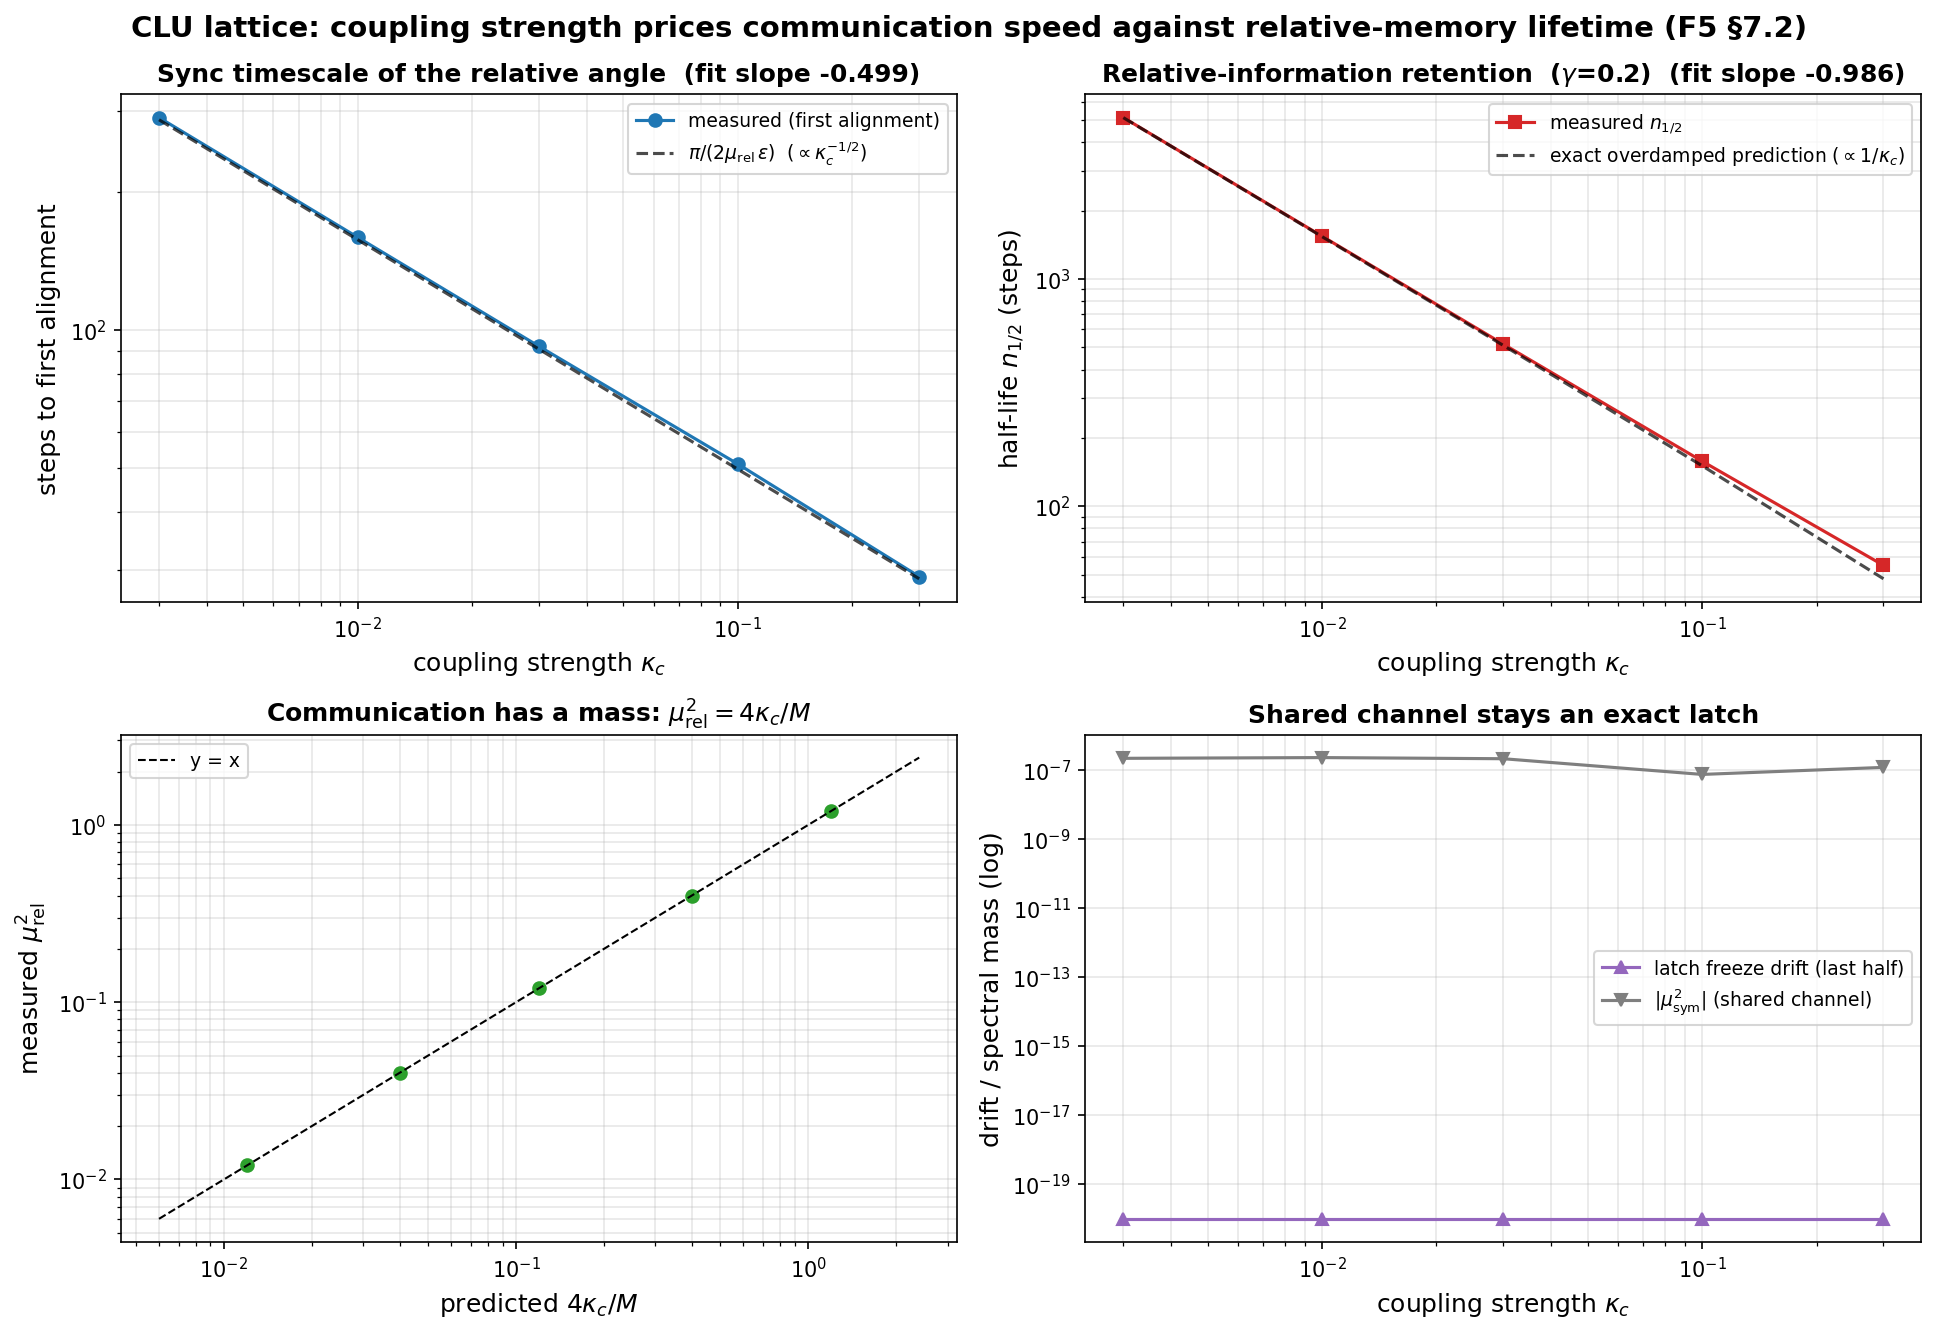
\includegraphics[width=0.7\linewidth]{figures/fig4_lattice_pricing.png}
\caption{\textbf{[verification] The communication price law, on a designed lattice.} Sweeping the static coupling $\kappa_c$ over two decades on a $2$-unit $SO(2)$ pair ($\gamma_{\rm probe}=0.2$, $\mathrm{dt}=0.05$, seed 42): synchronization time follows $\propto\kappa_c^{-1/2}$ (fitted slope $-0.499$) and relative-memory half-life $\propto\kappa_c^{-1}$ (slope $-0.986$), matching the theory note's predicted $-\tfrac12$/$-1$. Architecturally-invariant potential with analytic coupling $\Rightarrow$ \textbf{verification of the theory's exactness}, not a discovery (\texttt{v3-lattice-build}).}
\label{fig:pricelaw}
\end{figure}

\subsection{The interference firewall, measured: degree-bounded, not width-dependent (headline)}
\emph{(\textbf{Evidence}: lattices with learned MLP potentials. Sources: \texttt{v3-interference-extra} (12 seeds, $N\in\{2,4,6,8,12,16\}$, scaling + block-monolith controls; 8 seeds, 3 topologies) and \texttt{v3-interference-ntk} items 1--3 (3 seeds; $\kappa$-sweep, through-training). $2$-dim units, MLP potentials, $\kappa_c=0.05$, measured at initialization unless stated, laptop-CPU. \textbf{Headline = Figure~1.})}

The scaling credibility question is catastrophic interference: does updating one unit corrupt the others? We measure it. The operational interference of $A$ on $B$ is the \textbf{basin displacement} --- the force-field change over $B$'s block from a localized CD (wake/sleep) update on $A$, normalized by the intended change at $A$:
\[ R_{B\leftarrow A}=\frac{\lVert\Delta F|_B\rVert}{\lVert\Delta F|_A\rVert},\quad \Delta F=\nabla_qV_{\rm new}-\nabla_qV_{\rm old}\ \text{after}\ \theta\leftarrow\theta-\eta[\nabla_\theta V(\text{wake})-\nabla_\theta V(\text{sleep})]. \]
$R_{B\leftarrow A}=0$ iff $B$'s basin is untouched; the aggregate interference \emph{received} per unit is $S_B=\sum_{A\ne B}R_{B\leftarrow A}$ (we report $S=\mathrm{mean}_B S_B$). We compare the \textbf{modular lattice} against a \textbf{shared-potential monolith} (one $V_\theta:\R^{Nd}\to\R$ of the same family/width --- the honest ``no firewall'' baseline) and, below, against three \emph{block-diagonal} potentials that separate the two things ``modular'' could mean.

\paragraph{(i) The structural result: interference is confined to the coupling graph, exactly.} Across all $72$ modular runs ($6$ sizes $\times$ $12$ seeds), \textbf{every non-edge entry of $R$ is exactly zero in float32} --- $0$ nonzero of $4{,}656$ off-graph entries, against $4{,}656/4{,}656$ for the monolith. This is a structural identity, not a small number: wake and sleep configurations differ only in unit $A$'s block, so $\nabla_\theta[V(q_{\rm wake})-V(q_{\rm sleep})]$ vanishes identically on every own-potential $\theta_{V_B}$ ($B\ne A$) and on every coupling module not incident to $A$; only $\theta_{V_A}$ and the $\le\deg(A)$ couplings touching $A$ move. Hence
\[ S_B=\deg(B)\cdot\bar R_{\rm edge}, \qquad\text{verified } S/(\deg\cdot\bar R_{\rm edge})=1.000000 \text{ in every topology}\times N \text{ cell.} \]
\textbf{Per-unit received interference is bounded by the coupling graph's coordination number, not by the network's width.} A topology control makes this a measurement rather than an inference ($8$ seeds, $N\in\{4,8,16\}$):

\begin{center}\footnotesize\setlength{\tabcolsep}{4pt}
\begin{tabular}{lcccccc}
\toprule
topology & degree & $S(N{=}4)$ & $S(N{=}8)$ & $S(N{=}16)$ & slope $b$ (95\% CI) & $H_0\!:b=0$ \\
\midrule
chain & $1.50\to1.88$ & $7.93\times10^{-5}$ & $1.50\times10^{-4}$ & $1.15\times10^{-4}$ & $+0.264\pm0.171$ & $p=0.008$ \\
\textbf{ring} & $2.00$ & $1.19\times10^{-4}$ & $1.72\times10^{-4}$ & $1.32\times10^{-4}$ & $\mathbf{+0.071\pm0.183}$ & $p=0.391$ (flat) \\
\textbf{circulant-4} & $4.00$ & --- & $2.83\times10^{-4}$ & $2.64\times10^{-4}$ & $-0.066\pm0.315$ & $p=0.636$ (flat) \\
\bottomrule
\end{tabular}
\end{center}

Non-edge $R$ is exactly zero in \emph{every} topology, including the circulant, where graph distance and index distance disagree: the firewall follows the coupling graph, not the index layout. At fixed degree $S$ is \textbf{statistically flat in $N$} (ring); doubling the degree scales $S$ by $2.01\times$ at $N=16$ (the identity is exact per-run; the cross-arm ratio inherits the $\pm30\%$ init scatter of $\bar R_{\rm edge}$, so we quote the identity, never ``$2.0\times$'' as a constant).

\paragraph{We state the one residual preemptively.} A \emph{chain} is not degree-constant: its mean degree ramps $2(N{-}1)/N=1.0\to1.88$ over $N=2\to16$. Its $S$ therefore carries a small real positive slope ($b=+0.46\pm0.31$ over $N\in[2,16]$, 12 seeds; $+0.26\pm0.17$, $p=0.008$, in the 8-seed topology control), which a pure coordination effect predicts as $+0.289$ and which \textbf{vanishes under degree normalization} ($b(S/\deg)=+0.17\pm0.31$, consistent with $0$). We therefore never call a chain ``flat in $N$'': the claim is \emph{degree-bounded}, and the ring is where flatness is measured.

\paragraph{(ii) The growth result: degree-bounded vs width-linear (Figure~1).} With $12$ seeds and six sizes the arms' log-log slopes \textbf{diverge}: modular $b=+0.46\pm0.31$ vs monolith $b=+1.18\pm0.17$ (95\% CI, non-overlapping; Welch $p=3.3\times10^{-4}$, paired-by-seed $p=5.5\times10^{-4}$; monolith steeper in $11/12$ seeds). The modular curve saturates then decreases ($S(8)=1.32\times10^{-4}\to S(16)=1.13\times10^{-4}$, $b_{[8,16]}=-0.23\pm0.37$); the monolith keeps climbing ($b_{[8,16]}=+0.79\pm0.09$).

\begin{center}\footnotesize\setlength{\tabcolsep}{4pt}
\begin{tabular}{lcccccc c}
\toprule
arm & $N{=}2$ & $N{=}4$ & $N{=}6$ & $N{=}8$ & $N{=}12$ & $N{=}16$ & $b$ over $[2,16]$ \\
\midrule
\textbf{modular} (banded $\equiv$ uniform) & $6.41\mathrm{e}{-5}$ & $9.76\mathrm{e}{-5}$ & $1.24\mathrm{e}{-4}$ & $1.32\mathrm{e}{-4}$ & $1.12\mathrm{e}{-4}$ & $1.13\mathrm{e}{-4}$ & $+0.463\pm0.311$ \\
\textbf{monolith} (shared $V_\theta$) & $2.18\mathrm{e}{-1}$ & $6.40\mathrm{e}{-1}$ & $1.02$ & $1.34$ & $1.90$ & $2.32$ & $+1.184\pm0.170$ \\
\bottomrule
\end{tabular}
\end{center}

\noindent(mean $\pm$ s.d.\ over 12 seeds; separation $\times20{,}649$ at $N=16$.) The monolith's per-pair displacement is $\approx0.19$ with \textbf{no spatial structure}, and its aggregate crosses $S=1$ at $N\approx5.9$: \textbf{the aggregate cross-unit force perturbation a monolithic unit receives exceeds the magnitude of its own intended update} ($S(4)=0.640$, $S(6)=1.024$). We phrase this as force perturbation, not storage capacity: reading it as ``interferes with itself more than it stores'' would require the \emph{dynamical} interference half-life, which we have not measured (Appendix~C).

The modular residual leak is coupling-mediated: a $\kappa_c$-sweep ($N=4$, 3 seeds) gives log-log slope $1.99$, i.e.\ $\bar R_{\rm edge}\propto\kappa_c^2$, and \textbf{exactly $0$ at $\kappa_c=0$} --- a tunable price set by the coupling strength, not a fixed floor. The firewall is \textbf{mass-independent} --- banded and uniform lattices give \emph{bit-identical} $R$ ($\max|R_{\rm banded}-R_{\rm uniform}|=0.000\times10^{0}$ over $6$ sizes $\times$ $12$ seeds) --- and the separation \textbf{persists through training} where measured (2-unit lattices, 3 seeds: modular $R_{\rm off}$ $4.2\times10^{-5}\to8.9\times10^{-5}$ over epochs $0/150/300$; monolith $O(0.1$--$0.4)$ throughout; $N>2$ through-training unmeasured, Appendix~C).

\begin{figure}[t]
\centering
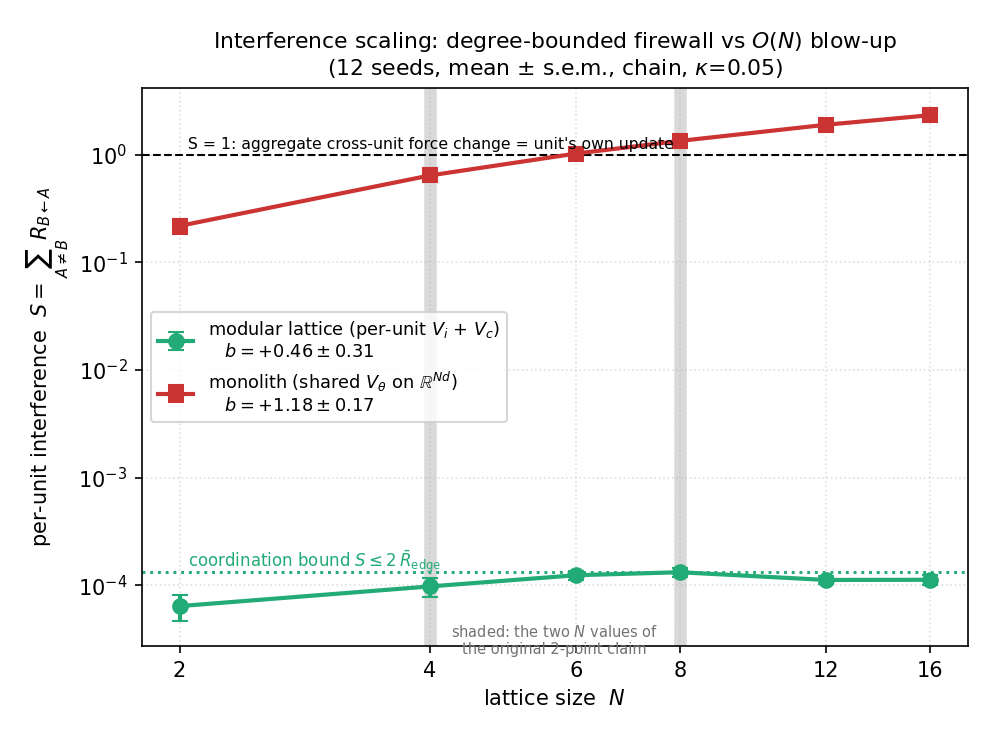
\includegraphics[width=0.78\linewidth]{figures/fig1_scaling_curve.png}
\caption{\textbf{[evidence] Headline: interference is degree-bounded, not width-dependent.} Per-unit received interference $S=\mathrm{mean}_B\sum_{A\ne B}R_{B\leftarrow A}$ vs lattice size $N$ (log--log; mean $\pm$ s.e.m.\ over \textbf{12 seeds}; chain, $\kappa_c=0.05$, 2-dim units, MLP potentials, at initialization, laptop-CPU). The shared-$V_\theta$ monolith is \textbf{width-linear} ($b=+1.18\pm0.17$) and crosses $S=1$ at $N\approx5.9$ (dashed: aggregate cross-unit force change equals a unit's own update). The modular lattice tracks the exact identity $S=\deg\cdot\bar R_{\rm edge}$ (its aggregate stays below $2\bar R_{\rm edge}$, dotted, because the chain's mean degree is $<2$) and saturates ($b=+0.46\pm0.31$ over $[2,16]$, entirely the chain's degree ramp $1.5\to1.88$; $b=-0.23\pm0.37$ over $[8,16]$); slopes diverge, Welch $p=3.3\times10^{-4}$. Shaded: the $N$ range accessible to a two-point measurement, shown to make explicit why two points could not separate these slopes (Appendix~G). On the rendered asset's title, the ``$O(N)$'' refers to the \textbf{monolith}, whose \emph{fitted} exponent is $1.18\pm0.17$; no arm of this paper's modular lattice is described as ``$O(1)$'' or ``flat in $N$'' in any figure or sentence. Source: \texttt{v3-interference-extra}.}
\label{fig:interference}
\end{figure}

\paragraph{(iii) What actually buys the firewall: parameter separation, not block structure.} A reviewer's first question is ``is this modularity, or did you just train $N$ nearly-separate networks?'' We answer with a control (12 seeds, $N\le16$): a \textbf{single} potential $V:\R^{Nd}\to\R$ with an explicitly block-diagonal Hessian, in three parameter-sharing regimes (full table + figures: Appendix~H).

\begin{center}\footnotesize\setlength{\tabcolsep}{3pt}
\begin{tabular}{lcccccc}
\toprule
arm & params ($N{=}2{\to}16$) & $S(N{=}8)$ & $S(N{=}16)$ & per-pair $\bar R$ & $b$ over $[2,16]$ & non-edge $R$ \\
\midrule
\textbf{block-untied} sep.\ $\theta_i$ & $2{,}370\to18{,}960$ & $\mathbf{0.0}$ & $\mathbf{0.0}$ & $\mathbf{0.0}$ & undef.\ ($S\equiv0$) & $0$ (exact) \\
\textbf{modular lattice} ($\kappa_c{=}0.05$) & $2{,}382\to19{,}112$ & $1.32\mathrm{e}{-4}$ & $1.13\mathrm{e}{-4}$ & ${\approx}6.5\mathrm{e}{-5}$ & $+0.46\pm0.31$ & $0$ (exact) \\
block-trunk (shared trunk) & $1{,}218\to1{,}680$ & $4.88\mathrm{e}{-1}$ & $1.05$ & $0.065$ & $+1.51\pm0.36$ & nonzero \\
monolith (cross-block $V_\theta$) & $1{,}253\to2{,}177$ & $1.34$ & $2.32$ & $0.19$ & $+1.18\pm0.17$ & nonzero \\
\textbf{block-tied} (deep-sets) & $1{,}185$ (const.) & $6.78$ & $1.45\times10^{1}$ & $\mathbf{0.97}$ & $+1.29\pm0.01$ & nonzero \\
\bottomrule
\end{tabular}
\end{center}

\textbf{Block structure alone recovers nothing:} \texttt{block-trunk} and \texttt{block-tied} have strictly block-diagonal Hessians and still show $O(1)$ per-pair interference and width-linear aggregate growth --- sharing \emph{any} parameters across blocks, even only a trunk, reopens the channel. \textbf{Block structure plus disjoint parameters recovers the firewall completely:} \texttt{block-untied} gives $S\equiv0$ \emph{exactly}, at every $N$ and every seed (diagonal $R[A,A]=1.000000$ throughout, so it is a genuine zero, not a dead self-response). \textbf{Interference is not a capacity effect:} the worst arm is the $1{,}185$-parameter tied potential (constant in $N$), the perfect arm the $18{,}960$-parameter untied one --- which kills the ``you just gave the modular arm more parameters'' confound in the cleanest way available.

The honest reading, which we prefer to the flattering one: \textbf{nothing physics-specific buys the firewall --- parameter separation does, and \texttt{block-untied} is a strictly \emph{better} firewall than our lattice} ($S\equiv0$ vs $\bar R_{\rm edge}\approx6.5\times10^{-5}$). The modular lattice \emph{is} \texttt{block-untied} plus an $O(\kappa^2)$ graph-local leak, and that leak is exactly the price of having a coupling graph at all ($0.0$ at $\kappa_c=0$). What the physics buys is that the lattice pays that price while retaining a \textbf{single joint symplectic Hamiltonian with priced, graph-local communication}: units that can talk, under one conservative dynamics, at a measured and bounded cost of talking (\S3.3). A network of disconnected potentials has a perfect firewall and nothing to say across it. Our monolith foil is correspondingly \emph{mild}: the permutation-equivariant deep-sets potential $V=\sum_if(q_i)$ --- a real architecture, not a strawman --- interferes $6.2\times$ harder in aggregate at $N=16$, with per-pair $\bar R=0.97$ (an update aimed at $A$ moves every other basin by ${\approx}97\%$ of the intended amount, the shared $f$ moving coherently at every block) and exceeds $S=1$ already by $N=4$. We report both foils and quote the naive monolith in the headline, which understates our case.

\emph{Metric discipline (Appendix~D):} the raw potential-NTK cosine is $\approx0.99$ for \emph{both} architectures and does not distinguish them; the firewall lives in the wake$-$sleep difference, which $R$ captures and the raw kernel does not. Report $R$, never the NTK cosine.

\subsection{The price list is predictive, not descriptive}
\emph{(\textbf{Evidence}: trained 2-unit lattices, prediction registered before measurement. Source: \texttt{v3-interference-ntk} item 2, $3$ seeds.)}

For each trained lattice we read $\keff$ from the \emph{learned} coupling potential alone (mass-weighted Hessian of $V_c$ along the relative mode, blind to any rollout) and \emph{then} predict recall horizon and sync from the price law; only after registering do we measure. Varying the static coupling makes $\keff$ span $91\times$:

\begin{center}\footnotesize\setlength{\tabcolsep}{4pt}
\begin{tabular}{lcccccc}
\toprule
$\keff$ (learned, blind) & sync \textbf{pred} & sync \textbf{meas} & $\lvert\Delta\rvert_{\rm sync}$/pred & $n_{1/2}$ \textbf{pred} & $n_{1/2}$ \textbf{meas} & $\lvert\Delta\rvert_{n_{1/2}}$/pred \\
\midrule
$0.0055$ & $210.9$ & $195$ & $7.5\%$ & $2773.4$ & $\infty$ (cens., $>11{,}600$) & --- \\
$0.0163$ & $123.1$ & $122$ & $0.9\%$ & $943.1$ & $1468$ & $55.7\%$ \\
$0.0556$ & $66.6$ & $68$ & $2.1\%$ & $273.9$ & $257$ & $6.2\%$ \\
$0.1602$ & $39.2$ & $41$ & $4.5\%$ & $92.9$ & $137$ & $47.5\%$ \\
$0.4970$ & $22.3$ & $23$ & $3.2\%$ & $27.5$ & $42$ & $52.8\%$ \\
\bottomrule
\end{tabular}
\end{center}

The \textbf{ranking is exact} --- Spearman$(n_{1/2}^{\rm pred},n_{1/2}^{\rm meas})=1.0$, Spearman$(\keff,n_{1/2}^{\rm meas})=-1.0$, both over $n=5$ lattices (exact $p=0.008$ under the null; the top-ranked, weakest-coupling lattice's $n_{1/2}$ is \textbf{right-censored} at $>11{,}600$ steps and enters as a near-latch, not a point measurement). Sync is predicted \textbf{pointwise to $\le7.5\%$ relative to the registered prediction} across the $91\times$ decade (residuals $\{7.5,0.9,2.1,4.5,3.2\}\%$; the maximum sits on the weakest-coupling lattice, $210.9$ predicted vs $195$ measured --- which is $8.2\%$ if one instead normalizes by the measured value, so we state the denominator). The \textbf{recall horizon $n_{1/2}$ itself is predicted in rank, not pointwise}: on the four \emph{uncensored} lattices its residuals are $\{55.7,6.2,47.5,52.8\}\%$ (the first-crossing scatter of a threshold-hitting-time observable), so we claim the \emph{ranking} of $n_{1/2}$ and the \emph{pointwise} value of sync, and nothing stronger. The measured $\keff$, read blind from coupling curvature, tells you which trained $2$-unit lattice has the longer recall horizon and its sync time before the task is run --- demonstrated pointwise at $N=2$, and, crucially, \textbf{not an $N=2$ artifact: the underlying price law holds flat in $N$ to $N\le16$} (Fig.~\ref{fig:pricinglaw}, next), so the priced channel spans the same range as the firewall.

\paragraph{The price list is not an $N=2$ artifact --- it holds flat in $N$ to $N\le16$ [verification, \texttt{v3-pricing-n-scaling}].} This is the designed-$SO(2)$/frozen-coupling testbed of Fig.~\ref{fig:pricelaw} (\S3.1) extended across $N$, so it is labeled \emph{verification of the theory's exactness across composition}, not a learned-system discovery; the learned-coupling arm is the control below. The underlying price law ($\text{sync}\propto\keff^{-1/2}$, $n_{1/2}\propto\keff^{-1}$) holds to its \textbf{pre-registered} tolerance not only at $N=2$ but at $N\in\{2,4,8,16\}$, \textbf{both chain and ring, $5$ seeds}, on U(1)-preserving (\texttt{channel\_spring}) trained lattices of designed $SO(2)$ units: fitted sync exponent $-0.49\pm0.02$ and $n_{1/2}$ exponent $-0.91\pm0.03$ (the $\approx-0.91$ vs $-1.0$ is the pre-registered first-crossing/kick-phase ripple), with $\mu_{\rm rel}^2$ residual $\le0.45\%$ and $R^2\ge0.998$, and --- the load-bearing observation --- \textbf{flat in $N$}, with no monotonic drift toward zero and $\keff$ exact against its analytic value at every $N$ (Fig.~\ref{fig:pricinglaw}). The prediction was registered before measurement. This closes the composition gap the firewall/price-list split otherwise opens (\S1,~\S5): the physics-specific priced channel now spans the \textbf{same} $N\le16$ range at which the degree-bounded firewall is established, rather than living at $N=2$. Appendix~C's earlier concession that the trained-lattice scaling exponent was ``inconclusive'' is now \textbf{attributed}, not merely retracted: it was an \textbf{artifact of the shipped random-$W$ coupling's $U(1)$ breaking}, which clusters $\keff$ into a $\le1.4\times$ range across a $100\times$ $\kappa$-target sweep so no exponent is fittable (control $R^2\le0.47$; App.~C), and the symmetry-preserving coupling resolves it --- the control's failure to fit is itself the \emph{explanation} of App.~C, not a weakness. \emph{Scope (C-5/C-6):} designed $SO(2)$ units, a \textbf{frozen $U(1)$-preserving \texttt{channel\_spring} coupling} (the one qualifier gating the exponent claim), $N\le16$, both topologies, $5$ seeds, wake-only training, laptop-CPU.

\begin{figure}[t]
\centering
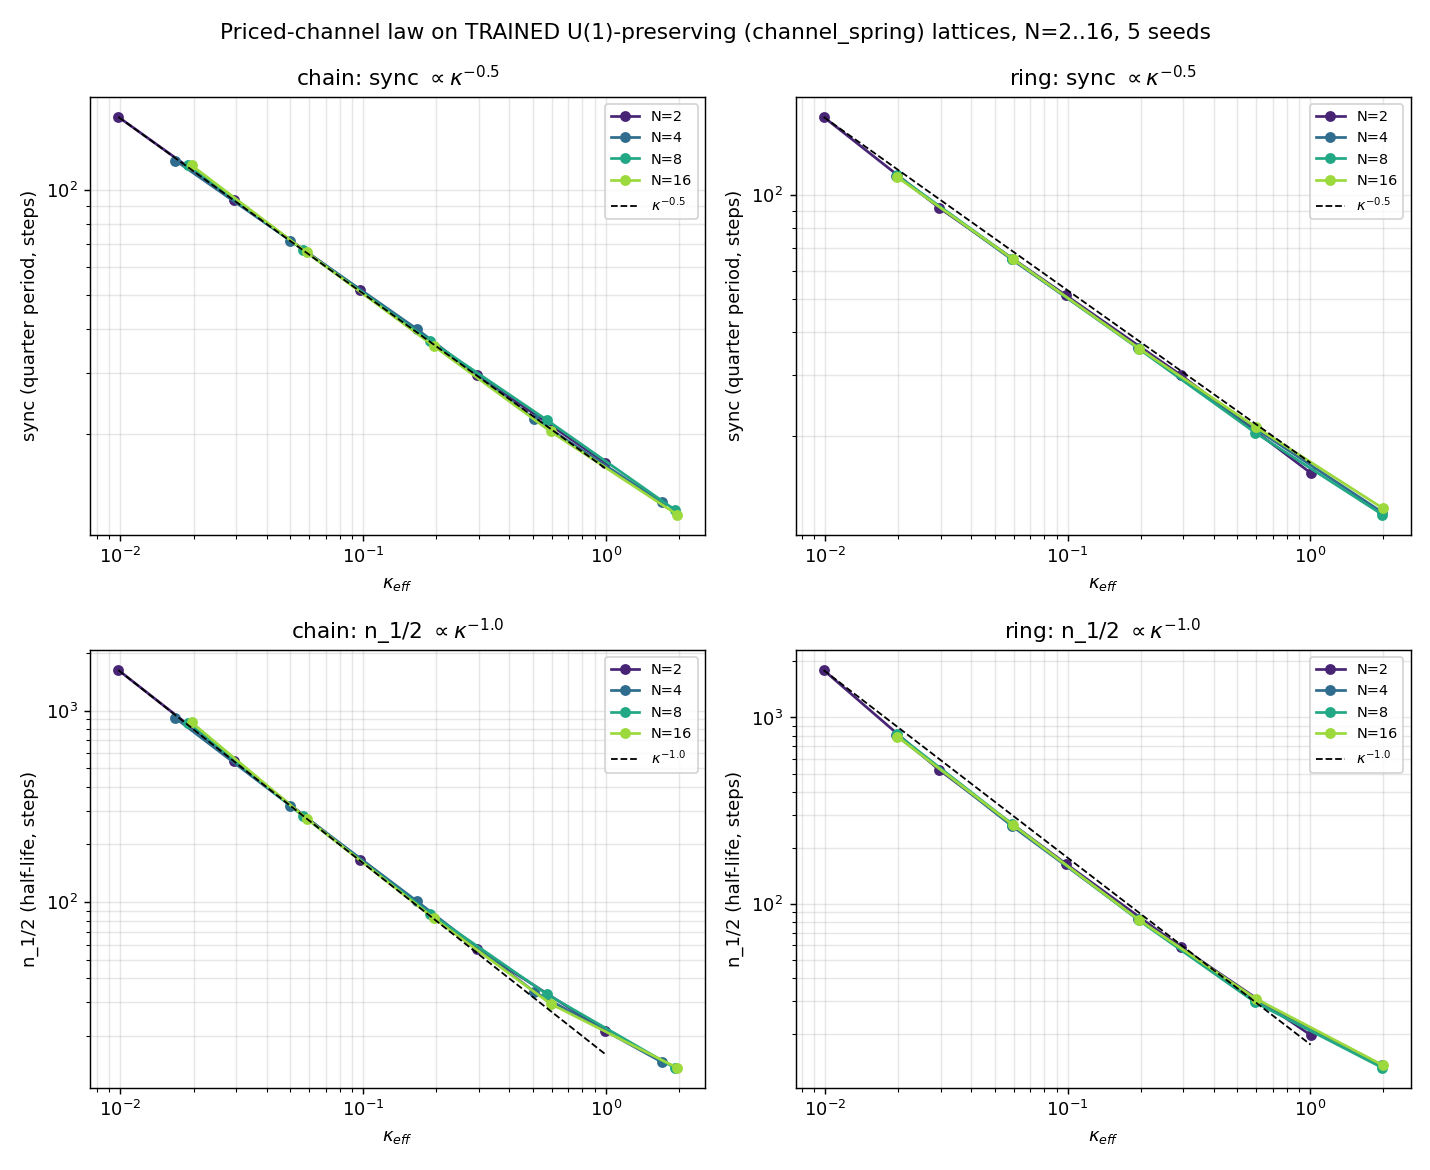
\includegraphics[width=0.78\linewidth]{figures/fig5_pricing_law_N.png}
\caption{\textbf{[verification] The price list holds flat in $N$ to $N\le16$.} Per-$N$ log--log fits of synchronization time and recall horizon $n_{1/2}$ against the blind-read $\keff$ on U(1)-preserving \texttt{channel\_spring} trained lattices of designed $SO(2)$ units, $N\in\{2,4,8,16\}$, chain and ring, $5$ seeds: the price-law slopes ($-0.49\pm0.02$ sync, $-0.91\pm0.03$ recall) are \textbf{flat in $N$} ($R^2\ge0.998$, $\mu_{\rm rel}^2$ residual $\le0.45\%$), so the law is not an $N=2$ artifact. Architecturally-invariant potential with a frozen $U(1)$-preserving coupling $\Rightarrow$ \textbf{verification of the theory's exactness across composition} (Fig.~\ref{fig:pricelaw} is the $N=2$ point of this same testbed). Pre-registered; predictions committed before measurement. Source: \texttt{v3-pricing-n-scaling}.}
\label{fig:pricinglaw}
\end{figure}

\begin{figure}[t]
\centering
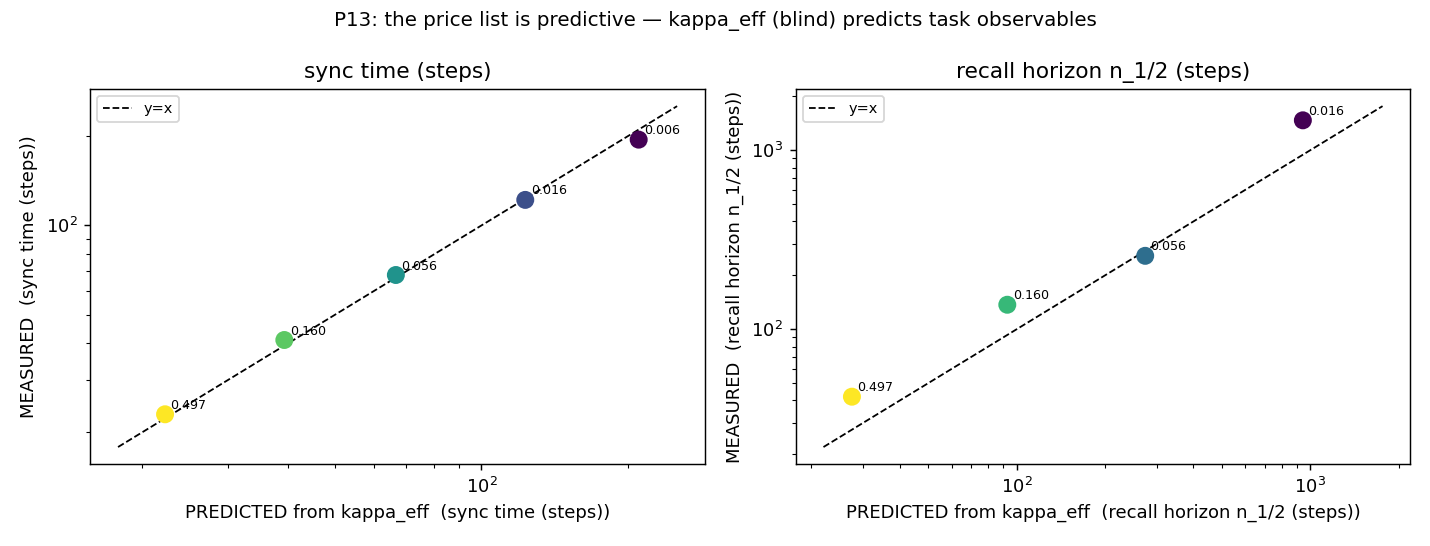
\includegraphics[width=0.6\linewidth]{figures/fig3_pricing_parity.png}
\caption{\textbf{[evidence] The price list is predictive.} Predicted vs.\ measured synchronization time across a $91\times$ $\keff$ decade on \emph{trained} $2$-unit lattices, $\keff$ read blind from the learned coupling potential and the prediction registered before measurement; points hug the parity line (max residual $7.5\%$ of the prediction; ranking exact, Spearman $1.0$). $3$ seeds, laptop-CPU (\texttt{v3-interference-ntk} item~2).}
\label{fig:pricing}
\end{figure}

\subsection{Banding as a method, not an oracle gift}
\emph{(\textbf{Evidence}: trained 2-unit ($16\times$-ratio) lattices, $5$ seeds (items 1--2)/$3$ seeds (item 3, $N\in\{2,4\}$). Source: \texttt{v3-band-selection} 1--3; \texttt{mass-lr-doctrine-test}. \textbf{Figure~2.})}

\textbf{(i) A wrong band costs.} Four arms spend the \emph{identical} log-spread budget, differing only in placement: matched, anti (inverted), orthogonal (spread on a no-signal axis), uniform. At $300$ ep, $5/5$ seeds,
\[ \text{matched }1.180 < \text{uniform }2.416 < \text{orthogonal }6.924 < \text{anti }12.791\quad(\text{held-out MSE}). \]
A correct prior is $0.49\times$ uniform; an inverted band of identical spread is $5.3\times$ worse than uniform, $10.8\times$ worse than matched. Banding is not ``any structure helps'' and not ``the answer for free.''

\begin{figure}[t]
\centering
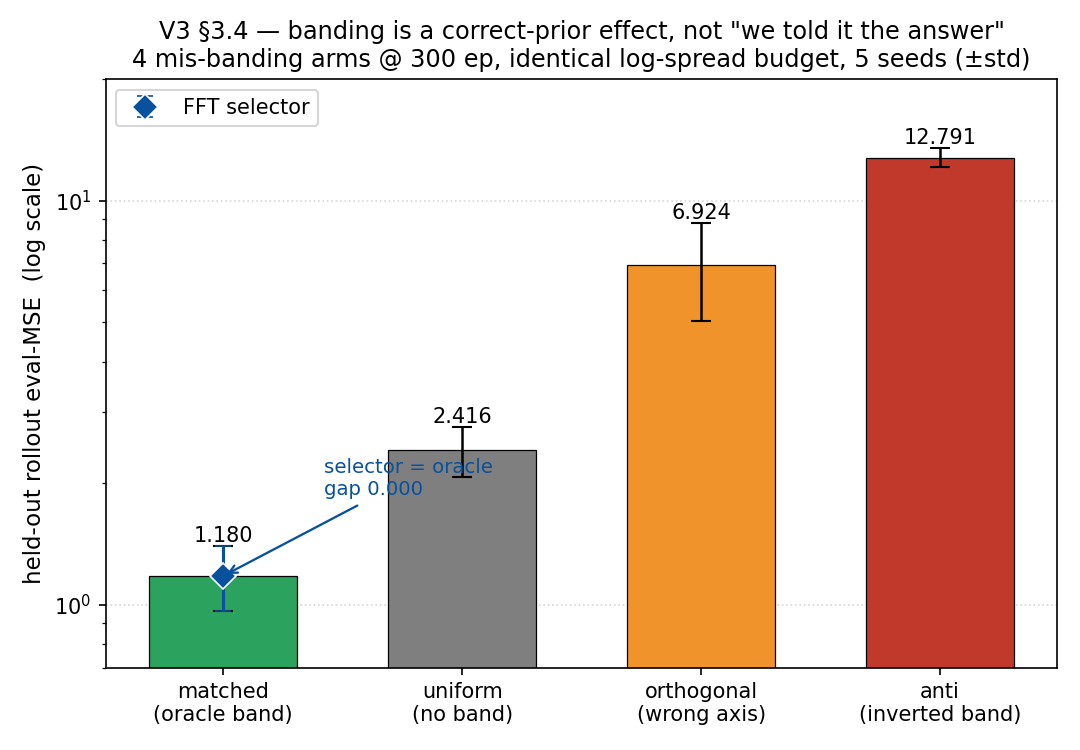
\includegraphics[width=0.62\linewidth]{figures/fig2_banding.png}
\caption{\textbf{[evidence] Banding is a correct-prior effect, not an oracle gift.} Held-out rollout MSE at $300$ epochs (log scale, $5$ seeds, $\pm$ s.d.) for four arms spending the \emph{identical} log-scale-spread budget on a $2$-unit lattice at $16\times$ ratio: matched (oracle band) $1.180\pm0.216$ $<$ uniform (no band) $2.416\pm0.345$ $<$ orthogonal (spread on a no-signal axis) $6.924\pm1.883$ $<$ anti (inverted band) $12.791\pm0.698$; matched beats every arm on $5/5$ seeds. Diamond: the from-data FFT selector lands on the oracle band (selector--oracle MSE gap $0.000\pm0.000$, $5/5$ seeds) --- \emph{when timescales are spectrally separable} (\texttt{v3-band-selection} items~1--2).}
\label{fig:banding}
\end{figure}

\textbf{(ii) The band is choosable from data --- with a stated qualifier.} A per-unit spectral (FFT) estimator maps each dominant frequency to $M_i\propto1/\omega_i^2$ and recovers the oracle band $[4.0,0.25]$ with \textbf{MSE gap $0.000\pm0.000$ on $5/5$ seeds}, one FFT over the training set. \emph{Qualifier:} the zero gap needs well-separated per-unit frequencies; on data whose timescales are not spectrally separable the gap opens --- ``cheap and exact \emph{when timescales are spectrally separable}.'' The optimizer-native alternative (induce-then-snap) is a fragile foil: correct ordering $4/5$ seeds, the single inversion pays the full mis-banded penalty (MSE $12.5$).

\textbf{(iii) The optimizer induces ordering, not magnitude.} Across $N\in\{2,4\}\times$ ratio $\in\{4\times,16\times\}$ ($3$ seeds, $1500$ ep), a mass-lr multiplier $\approx10$ reliably induces the correct ordering (alignment $+0.80$ to $+1.00$) and is the safe default; no induced run reaches the designed magnitude (designed fits $7$--$14\times$ better). A high multiplier ($\ge30$) is harmful in a \emph{ratio- and $N$-dependent} way: at $16\times$, mult $30$ \emph{degrades} the ordering ($+1.00\to+0.20$--$+0.33$) and $100\times$ \emph{inverts} it ($-1.00$ at $N=2$, $-0.20$ at $N=4$); at $4\times$ the ordering holds under $100\times$ but a global-mass runaway appears at $N=4$ (MSE $35.3\pm47.3$, $3$ seeds --- s.d.\ exceeds the mean, a seed-dominated single-run blow-up, not a characterized effect; at $N=2$, $4\times$, $100\times$ the order holds and MSE is $0.373$). Read the hierarchy off alignment/spread, \textbf{never MSE} (Appendix~E).

\subsection{Reversible $O(1)$-memory training}
\emph{(\textbf{Structural measurement on untrained models} --- a property of the integrator and autodiff graph, independent of parameter values, so not a learned-system claim. Source: \texttt{v3-reversible-o1} ($3$ seeds, float32 \textbf{and} float64), CPU, $D\le16$, laptop.)}

Because the CLU-Net's separable Hamiltonian gives the dissipative velocity-Verlet step a closed-form exact inverse, and the rollouts are already \texttt{lax.scan}-pure, at $\gamma=0$ training admits \textbf{exact recompute-backwards BPTT via analytic leapfrog inversion}: the backward pass reconstructs each previous state by the inverse map instead of storing the forward tape. Reconstructed gradients match standard stored-activation BPTT to $\le2.1\times10^{-6}$ relative in \textbf{float32} (the training default; $\le5.8\times10^{-15}$ in float64) at $T$ up to $1024$ --- five-plus orders below typical SGD gradient noise; whether that makes them \emph{training-indistinguishable} is \textbf{untested}, since these gradients have not yet been used to train (\S5). Peak activation memory is \textbf{$O(1)$ in sequence length vs $O(T)$}: at $T=1024,N=2$ the reversible pass uses $6.3$ KB against the standard $6.00$ MB --- a \textbf{$946\times$ reduction} --- the standard cost growing linearly in $T$ while the reversible cost stays flat (scaling only with state size). Wall-time is $\approx0.9\times$ standard (parity), but \textbf{only in the CPU / small-$D$ regime measured here} ($D\le16$, small potential MLP, laptop); on a GPU or with large potentials the recompute would likely surface as up to $\sim2\times$ overhead, so we claim parity only for this regime while the $O(T)\!\to\!O(1)$ \emph{memory} scaling is structural and does generalize.

\paragraph{Exact only at $\gamma=0$.} Any $\gamma>0$ makes the $(1-\gamma)$ contraction invertible only in exact arithmetic and amplifies reconstruction error as $(1-\gamma)^{-n}$, giving a \emph{finite} usable reversal horizon: $\approx3.3\times10^{4}$ steps at $\gamma=10^{-3}$ and $\approx5\times10^{2}$ at $\gamma=0.05$ (float64; $\sim100\times$ shorter in float32). This dovetails with the budget framing: the \textbf{reversibly-$O(1)$-trainable memory is exactly the conservative ($\gamma=0$) memory} --- \emph{reversibly-trainable memory is conservative memory} --- while dissipative segments fall back to stored activations or checkpointing (\S4). \emph{Scope (C-6):} this is the gradient mechanics only, on untrained models with a final-state loss; it is \textbf{not yet wired into the shipped \texttt{train\_chlu}} (windowed per-step loss), so a structural systems result, not yet a trained-lattice measurement (\S5).

\begin{figure}[t]
\centering
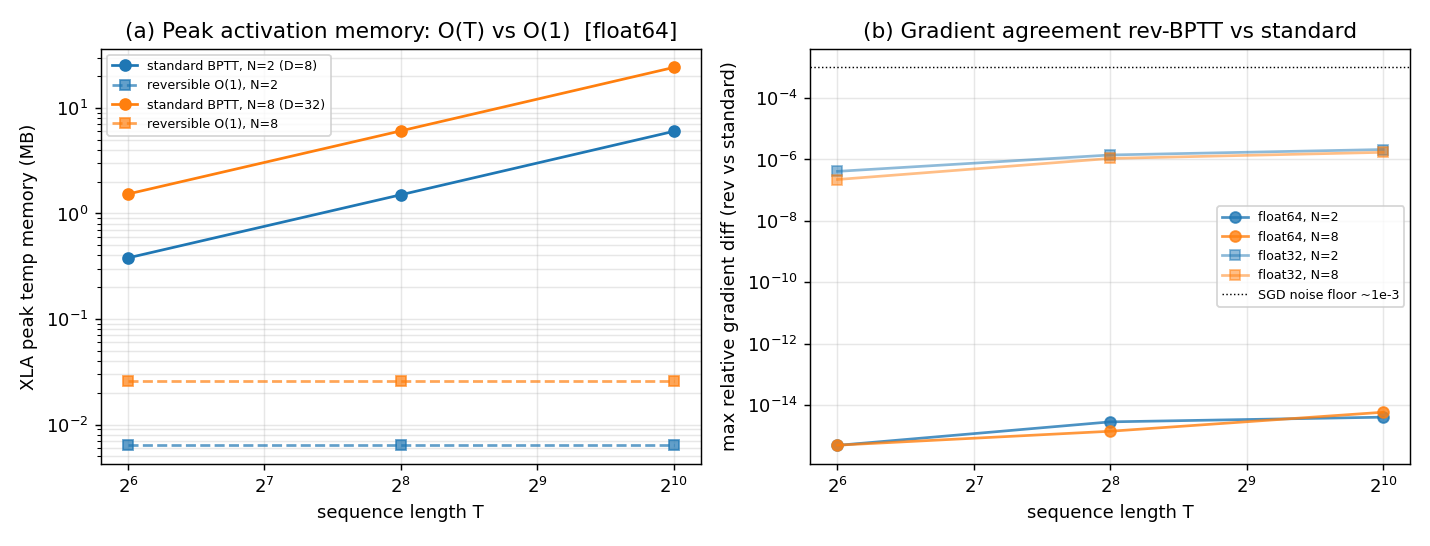
\includegraphics[width=0.85\linewidth]{figures/mem_grad_summary.png}
\caption{\textbf{[structural] Reversible $O(1)$-memory training ($\gamma=0$).} (left) peak activation memory vs.\ sequence length $T$: standard BPTT grows $O(T)$ while recompute-backwards stays flat $O(1)$-in-$T$ ($946\times$ at $T{=}1024,N{=}2$); (right) reconstructed-gradient relative difference vs.\ $T$ in float32/float64 ($\le2.1\times10^{-6}$ f32, $\le5.8\times10^{-15}$ f64 --- five-plus orders below typical SGD gradient noise; training-indistinguishability untested, \S5). \textbf{Structural measurement on untrained models} (a property of the integrator and the autodiff graph), CPU, $D\le16$, $3$ seeds; exact only at $\gamma=0$; the memory metric is the XLA compiler scratch estimate, a proxy for tape size rather than runtime peak RSS (Appendix~A.6). (\texttt{v3-reversible-o1}.)}
\label{fig:reversible}
\end{figure}

\subsection{The price of the physics prior, measured through the horizon}
\emph{(\textbf{Evidence}: learned MLP-potential controls, param-matched, on a \textbf{single CLU unit ($N=1$)} --- the price of the per-unit prior, not a lattice measurement. Source: \texttt{minus-the-physics} Part A; \texttt{fit-gap-anatomy} 1--3. Single unit ($N=1$), dim $2$--$4$, synthetic, laptop-CPU.)}

Symplectic volume conservation buys \textbf{bounded (BIBO) dynamics, a protected near-flat memory direction, and vacuum robustness under CD training}; the leapfrog structure buys the \textbf{latch}; the physics prior \textbf{costs raw fit}. Against a param-matched ($\pm0.05\%$) unconstrained twin and a broken-volume ablation: BIBO settled-fraction $1.00$ (CLU) / $0.33$ (broken-vol) / $1.00$ (twin); protected flat $\mu^2$ $0.008$ / $0.122$; latch coset drift $0.19$ (CLU) vs $1.15$ (twin, $\sim6\times$ looser); the vacuum \emph{survives} CD for the CLU where the broken-volume arm collapses to $r^*=0$. \emph{Two entries need care.} The BIBO claim is against the broken-volume ablation ($1.00$ vs $0.33$): the twin \emph{matches} the CLU's settle-fraction ($1.00$) on this short settle-probe but is bounded only empirically and \emph{diverges} on long rollout (MSE $196$ at $5000$ steps, Appendix~F.1), whereas the CLU is bounded by construction. The cost is specifically \textbf{contraction-forbidden} (volume; the broken-vol arm recovers $\approx2.4\times$ fit by \emph{leaking} volume), \textbf{not} the causal cap (inactive here): the twin fits $\approx15\times$ better ($0.013$ vs $0.190$). \emph{(These are the \texttt{minus-the-physics} dim-4 numbers; the recovery ladder in Appendix~F.2 uses a distinct circle-vacuum probe --- twin $0.0047$, CLU $0.207$, latch drift $0.778$ --- on a different testbed, not comparable digit-for-digit to the dim-4 pair here.)}

\paragraph{The loan is called at $\approx700$ steps.} Against the matched control on a stationary vacuum, the twin leads by $1$--$2$ orders out to $\approx500$ steps, is overtaken at $\approx700$, then diverges (cumulative MSE $196$ at $5000$ steps) while the CLU is the only arm flat \emph{by construction} (bounded plateau $0.20$--$0.23$). We claim the crossing and boundedness-by-construction; we do \emph{not} claim the lowest long-horizon plateau (broken-vol $0.14$, LSTM $0.13$ sit below CLU $0.22$). The \textbf{reach} term is real but secondary and aggregate-only: with the cap active it costs $+77\%$ MSE at $c=0.5$ and collapses to the uncapped baseline once $v_{\max}\ge$ required speed ($c\ge2$), with no per-step far-region concentration ($\mathrm{corr}(\text{err},|\dot q|)\approx0$).

\paragraph{Paid mechanisms rent back specific cheats (not interchangeable).} On the circle-vacuum probe (Appendix~F.2), a \textbf{global $\gamma$} recovers \textbf{$92\%$ of the \emph{absolute} contraction-forbidden fit gap, with BIBO, latch, and $\mu^2$ all preserved} ($\det J=(1-\gamma)^d$); the recovered unit still \textbf{trails the twin by $\approx4.6\times$ in ratio} ($0.0216$ vs $0.0047$ eval-MSE), but is bounded by construction (V2's exact wording for this shared number). A position-gated field $\gamma_\varphi$ does \emph{not} recover fit ($-24\%$) --- the wrong lever. A squeeze $S^{(M)}$ rents reach with an exact \textbf{matched-quadratic-$H$ certificate} (oracle placement; $\det=1$ to $3\times10^{-7}$, injection $\le e^{2|\zeta|}$, $\zeta=1$ grants $\Delta q=2.18>2.0$). Ladder + negatives: Appendix~F.

\section{Related work}
\textbf{Hamiltonian and symplectic recurrence (home turf).} Our unit is a \emph{learned-Hamiltonian, symplectically-integrated} recurrent cell, so the nearest architectural cousin is the \textbf{Symplectic Recurrent Neural Network} (Chen, Zhang, Arjovsky \& Bottou, 2020), which learns a Hamiltonian and advances it with a symplectic integrator under multi-step training; Hamiltonian and Lagrangian Neural Networks (Greydanus, Dzamba \& Yosinski, 2019; Cranmer et al., 2020) learn the energy from data, while stability-oriented recurrences --- Lipschitz RNNs (Erichson et al., 2021) and the coupled-oscillator coRNN (Rusch \& Mishra, 2021) / LEM (Rusch et al., 2022) --- engineer bounded dynamics without a symplectic form. The classic gated baseline our Appendix~F.1 compares against is the LSTM (Hochreiter \& Schmidhuber, 1997). Against all of these our contribution is deliberately orthogonal: \textbf{not a better single cell but a \emph{composition law} for many such cells} --- the measured interference firewall (\S3.2), the coupling price list (\S3.3), and the reversible-$O(1)$ corollary (\S3.5) are statements about \emph{coupling} learned-Hamiltonian units into a lattice, a regime none of the single-cell works address. The conformal-symplectic (damped-leapfrog) structure and its $h<2$ stability limit are standard for dissipative geometric integrators (Hairer, Lubich \& Wanner), read here as \emph{memory} statements for a learnable $H$. \textbf{Symmetry and memory lifetime.} Mo (2026) proves an exactly equivariant recurrent \emph{flow} has $\dim(G/H)$ zero Lyapunov exponents and that a ``pseudo-gap'' predicts a finite lifetime --- the \emph{kinematics} of protection, silent on what \emph{sets} the gap; our lattice supplies a constitutive, mass-controlled gap and a measured account of how protection composes across many coupled units. \textbf{Geometry-first structured recurrence.} A line engineers recurrence from a chosen symmetry (Di Bernardo et al.; Keller); we headline the \emph{pricing/budget} consequences of a coupling, not ``we choose $G/H$.'' \textbf{Modular vs. monolithic sharing.} Catastrophic interference --- overwriting stored function when a distributed network learns new content --- has been understood since McCloskey \& Cohen (1989) and French (1999) as a consequence of \emph{shared} representations. Two remedy families exist. The first \emph{prevents} interference by construction: modular architectures and mixtures-of-experts route content to different parameters (Jacobs et al., 1991; Shazeer et al., 2017), and parameter-isolation continual learners freeze or mask per-task subnetworks (Kirkpatrick et al., 2017; Mallya \& Lazebnik, 2018). The second \emph{measures} interference to minimize it during optimization: the NTK-overlap matrix quantifies cross-task forgetting (Doan et al., 2021), and gradient-alignment/gradient-surgery methods treat conflicting (negative-inner-product) updates as the signal to suppress (Riemer et al., 2019; Yu et al., 2020). Our lattice sits at the intersection: interference between units is neither merely prevented nor globally minimized but \emph{measured as a coupling-resolved kernel}. A shared-potential monolith moves every other unit's basin by $\approx0.19$ per update, unstructured and \textbf{width-linear} ($N^{1.18\pm0.17}$); the modular lattice moves a graph neighbour by $\approx6.5\times10^{-5}$ and a non-adjacent unit by \emph{exactly} zero, the leak $\propto\kappa^2$ (zero at $\kappa=0$) --- an architectural \textbf{degree-bounded vs.\ width-linear} separation and explicit coupling power-law, a \emph{priced}, graph-local firewall rather than the diffuse, data-dependent overlap on monoliths (Doan et al., 2021) or the sample-complexity separation for modular tasks (Boopathy et al., 2025). Our controls locate the mechanism precisely, and not where a physics-first reading would put it: \textbf{parameter separation, not block structure or geometry, closes the channel} --- a block-diagonal potential with tied parameters (a permutation-equivariant, deep-sets-style summed potential) interferes \emph{worse} than the unstructured monolith, while the same potential with per-block parameters gives exactly zero interference. Our firewall is thus the parameter-isolation family's guarantee (Kirkpatrick et al., 2017; Mallya \& Lazebnik, 2018) obtained \emph{by construction} rather than by penalty or mask; what the joint Hamiltonian adds is not a better firewall but a \textbf{priced channel through it} (\S3.3), so that units may communicate under a single conservative dynamics at a coupling cost that is measured, graph-local and $O(\kappa^2)$. \emph{(Scope: 2-dim units, chain/ring/circulant-4, MLP potentials, $N\le16$, $\kappa=0.05$, 8--12 seeds, measured at initialization; \S3.2, Appendices~D and~H.)} \textbf{Reversible / $O(1)$-memory training.} Trading stored activations for recomputation is the standard route to memory-cheap backprop: gradient checkpointing recovers activations at $O(\sqrt T)$ memory, and reversible architectures (RevNet / momentum-net / reversible-integrator lineage) reconstruct them exactly at $O(1)$ by an invertible forward map. The damped-symplectic lattice is invertible for the \emph{physics} reason that a separable Hamiltonian's leapfrog step has a closed-form inverse; \S3.5 \emph{measures} the resulting trade (exact $O(1)$-in-$T$ memory at $\gamma=0$, float-indistinguishable gradients) and makes explicit the boundary the general framing hides: exactness holds only along the conservative direction, so a network interleaving $\gamma>0$ blocks must checkpoint those segments. Positioning against the checkpointing $O(\sqrt T)$ middle-ground and accelerator-scale measurement are open (\S5). \emph{(Specific published anchors --- checkpointing, RevNet/momentum-net --- to be finalized from the scout bibliography.)}

\section{Limitations and horizon}
\textbf{Scope.} Every learned-system number is on $2$-dim units, MLP potentials, laptop-CPU, synthetic two-timescale data: $N\le16$ and $8$--$12$ seeds for interference, $N\le8$ and $3$--$5$ seeds elsewhere; industrial-scale and real-data behavior are untested (the largest gap). \textbf{The composition, owned (so no reviewer has to assemble it).} Two facts sit far apart in this paper and a reader will compose them, so we do it here. \emph{(a)} The interference firewall is our headline but \textbf{not our physics}: a potential of disjoint per-unit parameter blocks is a strictly better firewall than our lattice ($S\equiv0$ vs $\bar R_{\rm edge}\approx6.5\times10^{-5}$, \S3.2(iii)) with no Hamiltonian at all --- \emph{parameter isolation}, not the symplectic structure, confines interference. \emph{(b)} Our physics-specific claim is the \textbf{priced channel} (\S3.3), and it is \textbf{no longer stranded at $N=2$}: its predictive parity is demonstrated on trained $2$-unit lattices with \emph{learned} couplings (evidence, \S3.3), and the underlying price law is now \textbf{verified to hold flat in $N$ at $N\in\{2,4,8,16\}$}, both topologies, on the designed-$SO(2)$/frozen-$U(1)$-preserving-coupling testbed --- the same substrate as the $N=2$ verification (\S3.1), extended across composition (Figs.~\ref{fig:pricinglaw}--\ref{fig:exponentN}; pre-registered, $5$ seeds). Appendix~C's earlier ``inconclusive on trained lattices'' is resolved: it was an \textbf{artifact of a symmetry-breaking coupling} (a \emph{learned} random-$W$ coupling clusters $\keff$ into a $\le1.4\times$ range so no law is fittable), which the $U(1)$-preserving coupling fixes --- the control's failure is the \emph{explanation}, not a weakness. Composed: the degree-bounded firewall is established (evidence) at $N\le16$, and the priced channel it lets through is now verified across the \textbf{same} $N\le16$ range, so the composition gap is closed --- the physics-specific contribution spans the firewall's range rather than living at $N=2$. The residual honest scope: the exponent's cross-$N$ authority is the designed testbed (as at $N=2$), and reading the \emph{fitted exponent} off freely-\emph{learned} couplings at $N>2$ (rather than the ranking/parity map, which already survives learning) remains a follow-up --- but no main-text claim now bounds on an $N=2$ limitation. The thesis composes without a residual: \textbf{modularity is the firewall; a single joint symplectic Hamiltonian is what lets the modules talk, at a price we measure --- across the full range at which the firewall is established.} \textbf{Certificate altitude.} The ``exactly zero'' beyond the graph is a property of the position-only coupling and the locality of the contrastive update (it holds on chain, ring and circulant-4 graphs, and is analytic, not fitted); it is measured on the potential NTK (basin displacement $\Delta F$), not a full attractor re-settle, so the $S=1$ crossing is force perturbation and not storage, and the \emph{dynamical interference half-life} is \textbf{unmeasured} (Appendix~C). Interference is measured \textbf{at initialization}: the exact zeros are training-invariant by construction, but $\bar R_{\rm edge}\approx6.5\times10^{-5}$ is an init-scale quantity and through-training persistence is measured only at $N=2$. A \emph{trajectory-mediated} interference channel is \textbf{unmeasured}. The arms are not parameter-matched ($19{,}112$ modular vs $2{,}177$ monolith at $N=16$); the confound is bounded rather than eliminated by the block-tied ($1{,}185$ params, worst) / block-untied ($18{,}960$ params, zero) controls. The $\propto\kappa^2$ leak law is established at $N=4$ only. The pricing prediction is on $2$-unit trained lattices; the selector's zero gap is contingent on spectral separability; the wormhole edge is built and $C^1$ but not shown to beat a dense-MLP baseline, and the intra-unit wormhole is a design hypothesis. \textbf{Reversible-training scope.} The $O(1)$-memory result (\S3.5) is the gradient mechanics on \emph{untrained} models with a final-state loss on CPU; it is \textbf{not yet wired into \texttt{train\_chlu}}, the wall-time parity is CPU/small-$D$ only, and exactness is $\gamma=0$-only --- wiring it into the real trainer, an accelerator (GPU/HBM) memory + honest wall-time measurement at $T\gtrsim4\mathrm{k}$ where standard BPTT OOMs, and a gradient-checkpointing ($O(\sqrt T)$) Pareto baseline are the load-bearing follow-ups. \textbf{Horizon:} those reversible follow-ups; through-training interference at $N\in\{4,8,16\}$ and a parameter-matched monolith; a $\kappa$-sweep at $N=16$ to close $S=\deg\cdot c\,\kappa^2$ into a closed-form price for the firewall; 2-D grid and small-world topologies (where a wormhole edge should add exactly its own degree contribution --- a \emph{quantitative price for a wormhole}); the irrep firewall; real-data banding.

\appendix
\section{Flag-provenance tables (C-7)}
All results laptop-CPU, JAX; numbers transcribed from source reports. \textbf{A.1 CLU-Net (\S3.1, \texttt{v3-lattice-build}, verification):} commits \texttt{c124103}/\texttt{9c39b12}/\texttt{79dcac9}; chain, \texttt{SpringCoupling} (static $\kappa_c$); pricing run designed $SO(2)$ pair $\gamma_{\rm probe}=0.2$, seed 42, $f32$, $\kappa_c\in\{0.003,0.01,0.03,0.1,0.3\}$; $x64$ tests; scaling smoke $N\in\{2,4,8\}$. \textbf{A.2 Firewall, $\kappa$-sweep and through-training (\S3.2, \texttt{v3-interference-ntk}):} \texttt{9a13455}, chlu 0.2.4, seeds $\{0,1,2\}$; unit\_dims $[2]\times N$, \texttt{mlp} hidden 32, \texttt{newtonian\_learned}; monolith \texttt{CHLU(dim=2N)}; probe $\eta=0.05$, $r=0.5$; $\kappa=0.05$, sweep $\{0,0.01,0.03,0.1,0.3\}$ at $N=4$; through-training epochs $\{0,150,300\}$ at \emph{$N=2$}. \emph{Supersession:} this run's $N\in\{4,8\}$, 3-seed scaling numbers are superseded for the \emph{growth} claim by A.2b (12 seeds, 6 sizes); the two harnesses agree bit-exactly on the shared cells (max rel diff $0.00\times10^{0}$), so differences are seed sampling, not metric drift (Appendix~D.1). \textbf{A.2b Interference scaling, topology and block-monolith controls (\S3.2(i)--(iii), \texttt{v3-interference-extra}, evidence):} commit \texttt{37dc664}, repo read-only (\texttt{git status --porcelain} empty before \& after); main venv, \textbf{JAX 0.9.0}, CPU (\texttt{CpuDevice(id=0)}), equinox, chlu 0.2.4, scipy 1.17.0, x32 default precision; seeds $\{0\ldots11\}$ (12) for scaling/block, $\{0\ldots7\}$ (8) for topology; $N$ grid $\{2,4,6,8,12,16\}$ (scaling/block), $\{4,8,16\}$ (topology); \texttt{build\_lattice}, unit\_dims $[2]\times N$, \texttt{mlp} hidden 32, \texttt{newtonian\_learned}, \texttt{spring} coupling, coupling\_dim 2, proj\_init\_scale 0.1, $\kappa_c=0.05$, edges chain (default)/ring/circulant-4; banding \texttt{mass\_scales} $=4.0$ (even) / $0.25$ (odd), uniform $=$ None; monolith \texttt{CHLU(dim=2N,hidden=32)}; block monoliths: single $V:\R^{2N}\to\R$, per-block MLP \texttt{Linear(2,32)$\to$tanh$\to$Linear(32,32)$\to$tanh$\to$Linear(32,1)} $+\,0.05\lVert q\rVert^2$ (mirrors \texttt{PotentialMLP}), regimes \texttt{block\_untied}/\texttt{block\_trunk}/\texttt{block\_tied}; probe = \emph{identical code path} to A.2 (\texttt{force\_interference} imported verbatim), $\eta=0.05$, $r_{\rm probe}=0.5$, all units at memory loci, only $A$ perturbed (wake $=m_A$, sleep $=m_A+0.6\mathcal N$), $R$ row-normalized by $R[A,A]$; measurement at \textbf{initialization} (no training in this run); NTK cosine not computed; non-defaults \texttt{kinetic=newtonian\_learned} (banding needs \texttt{log\_mass}), training config inapplicable; \emph{metric-identity anchor}: re-running this harness on seeds $\{0,1,2\}$ at $N\in\{4,8\}$ reproduces \texttt{v3-interference-ntk/interference\_init.json} to max relative difference $0.00\times10^{0}$ (bit-exact) for both arms; statistics = per-seed OLS of $\log_{10}S$ on $\log_{10}N$, mean $\pm$ 95\% CI over seeds ($t$, dof 11), Welch and paired-by-seed $t$-tests for the slope difference. \textbf{A.3 Pricing (\S3.3):} wake-only, lr $10^{-3}$, $x64$, $\kappa_{\rm static}\in\{0.01,0.03,0.1,0.3,1.0\}$, 200 ep. \textbf{A.3b Price law flat in $N$ (\S3.3, Figs.~\ref{fig:pricinglaw}--\ref{fig:exponentN}, \texttt{v3-pricing-n-scaling}, verification across composition, pre-registered):} commit \texttt{e3c8931} (main), JAX 0.9.0, CPU, $x64$; wake-only (sleep off), $M=1$, $\mathrm{dt}=0.05$, 60 ep, window 128, $\gamma=0$ (sync)/$\gamma_{\rm probe}=0.2$ ($n_{1/2}$); designed $SO(2)$ MexicanHat units ($f{=}M{=}\lambda{=}1$, start at analytic vacuum, $\keff$ $0.1981\to0.1983$ over 60 ep); \emph{primary} \texttt{channel\_spring} ($U(1)$-preserving, frozen), $N\in\{2,4,8,16\}\times\{$chain,ring$\}\times\kappa_{\rm target}\in\{0.01,0.03,0.1,0.3,1.0\}\times$ seeds $\{0\text{--}4\}$ (198/200 rows; ring/$N{=}16$/$\kappa{=}1.0$ is 3 seeds, $\pm0.014$); \emph{control} \texttt{spring\_random} (legacy random-$W$, $U(1)$-breaking, trainable $W$, static $\kappa_S=0.1$), chain, 100 rows; extractor $\keff=\tfrac14 M\lambda_{\max}=0.5\kappa\lambda_{\max}(L)$ (5-dp identity); pre-registered decision rule (HOLDS iff $s_N\in[-0.55,-0.45]$, $h_N\in[-1.15,-0.80]$ $\forall N$, no drift, $\mu_{\rm rel}^2<2\%$) applied verbatim; non-defaults \texttt{coupling\_type=channel\_spring}, langevin n/a (wake-only). \textbf{A.4 Banding (\S3.4):} band-selection \texttt{9a13455}, module \texttt{c4bc004} (additive), \texttt{mass\_lr\_mult}$\in\{1,3,10,30,100\}$, seeds items 1/2 $\{0..4\}$, item 3 $\{0,1,2\}$; \emph{env caveat}: band-selection worktree JAX 0.10.2 vs main 0.9.0 (headline numbers version-stable, reproduce \texttt{b1782b0} bit-for-bit); mass-lr \texttt{db3369b}, commits \texttt{be12b73}/\texttt{df11483}, data masses $[4.0,0.25]$. \textbf{A.5 Price of physics (\S3.6):} minus-physics \texttt{db3369b} (\texttt{9533ef3}/\texttt{c33b41f}/\texttt{b41410f}), dim 4, hidden 64, \texttt{mlp}, 150 ep, seeds $\{42,43,44\}$, wake-only, sleep\_friction 0; fit-gap \texttt{9a13455}; param match chlu 4549 / broken\_volume 4557 / twin 4551. \textbf{A.6 Reversible $O(1)$ (\S3.5, \texttt{v3-reversible-o1}, structural):} commit \texttt{63fea62} (main @ wave-6), JAX \textbf{0.9.0}, device cpu, repo read-only (inverse map reconstructed from $H$, validated against the shipped \texttt{velocity\_verlet\_step}); item 1 \texttt{CHLU(dim=8,hidden=16)}, \texttt{newtonian\_learned}, \texttt{mlp}, \emph{untrained} random init, $\gamma\in\{0,10^{-4},10^{-3},10^{-2},0.05,0.1,0.3\}$, float32 \textbf{and} float64, $T$ to $16384$; item 2 \texttt{build\_lattice([2]$\cdot$N)} $N\in\{2,8\}$ hidden 16, spring $\kappa_c=0.05$, chain, seeds $\{0,1,2\}$, final-state MSE, $T\in\{64,256,1024\}$, \emph{untrained}; memory via XLA \texttt{memory\_analysis().temp\_size\_in\_bytes} (compiler estimate, deterministic; proxy for tape size); grad rel-diff $\le2.1\times10^{-6}$ (f32)/$\le5.8\times10^{-15}$ (f64) @ $T{=}1024$; peak temp $6.00$ MB vs $6.34$ KB ($946\times$, $N{=}2$), $24.20$ MB vs $25.7$ KB ($940\times$, $N{=}8$); wall-time $0.86\times$ (f64)/$0.94\times$ (f32); $\gamma{>}0$ f64 horizons $\ge1.3\mathrm{e}5$/$3.3\mathrm{e}4$/$4.1\mathrm{e}3$/$5.1\mathrm{e}2$/$1.3\mathrm{e}2$ at $\gamma=10^{-4}/10^{-3}/10^{-2}/0.05/0.1$ ($\sim100\times$ shorter f32). \emph{Scope:} untrained + final-state loss (not the shipped windowed trainer), CPU $D\le16$; wall-time regime-specific; memory scaling structural.

\section{The mis-banding price panel and over-lr failure modes (C-9)}
\textbf{B.1 Degradation curve ($5$ seeds, \texttt{v3-band-selection} item 1):}
\begin{center}\small
\begin{tabular}{lcccc}
\toprule
budget & matched & uniform & orthogonal & anti \\
\midrule
60 ep & $2.812\pm0.327$ & $3.751\pm0.336$ & $8.874\pm2.198$ & $14.905\pm0.686$ \\
300 ep & $\mathbf{1.180\pm0.216}$ & $2.416\pm0.345$ & $6.924\pm1.883$ & $12.791\pm0.698$ \\
\bottomrule
\end{tabular}
\end{center}
matched beats every arm $5/5$ seeds at both budgets ($300$-ep ratios $0.488$/$0.170$/$0.092$). \textbf{B.2 Selection recipe (item 2):} uniform $2.416\pm0.345$; oracle $1.180\pm0.216$; \textbf{selector $1.180\pm0.216$ (gap $+0.000\pm0.000$)}; masslr-init $3.527\pm4.493$ (ordering $4/5$; seed-2 inversion $\to$ MSE $12.5$). \textbf{B.3 Over-lr (N8/N9):} at $16\times$, $100\times$ lr $\to$ alignment $-1.00$, unitM $(3.90,5.34)$, \emph{lowest} MSE $0.324$ (a trap --- N8); at $4\times$, $100\times$ lr $\to$ global runaway MSE $35.3\pm47.3$; slow-first curriculum did not help (align $-0.54\pm0.72$; N9). Safe point: multiplier $\approx10$.

\section{Honest unmeasured list (open items)}
\emph{Trajectory-mediated banding channel} (banding changes which loci drive updates --- unmeasured); \emph{irrep firewall} (does the NTK factor across irreps? --- unmeasured); \emph{block-structured monolith} --- \textbf{now MEASURED} (\S3.2(iii), Appendix~H): it is the separate \emph{parameters}, retained here as a record of the item's discharge; \emph{dynamical interference half-life} (we map $\Delta F$, not the event's dynamical half-life --- unmeasured; the one thing still blocking a \emph{storage} reading of the $S=1$ crossing); \emph{through-training interference at $N>2$} ($R$ measured at init for $N\le16$; exact zeros training-invariant by construction, but $\bar R_{\rm edge}$ is init-scale and only $N=2$ was tracked to 300 epochs --- unmeasured at $N\in\{4,8,16\}$); \emph{parameter-matched monolith} ($19{,}112$ vs $2{,}177$ params at $N=16$; capacity is decoupled from interference by the tied/untied pair, but a width-matched sweep is unrun); \emph{$\kappa$-sweep beyond $N=4$} (would close $S=\deg\cdot c\,\kappa^2$ into a closed-form price --- unmeasured); \emph{non-MLP potentials and richer graphs} (no \texttt{so2\_invariant}/\texttt{deep\_mlp}; no 2-D grid or small-world topologies --- unmeasured); \emph{trained-coupling scaling exponent} --- \textbf{now RESOLVED} (N16; \S3.3, Figs.~\ref{fig:pricinglaw}--\ref{fig:exponentN}, \texttt{v3-pricing-n-scaling}): the earlier ``inconclusive'' is attributed to the shipped random-$W$ coupling's $U(1)$ breaking (clusters $\keff$ to a $\le1.4\times$ range, control $R^2\le0.47$, exponents $\pm12$ to $\pm887$), \emph{not} a physics degradation; on a $U(1)$-preserving \texttt{channel\_spring} coupling (designed $SO(2)$ units, frozen coupling) the exponent is \textbf{verified flat across $N\le16$} ($-0.49\pm0.02$ / $-0.91\pm0.03$, both topologies, $5$ seeds, pre-registered) --- the $N$-extension of the \S3.1 verification --- so the ``inconclusive'' is understood as a property of the \emph{learned} symmetry-breaking coupling, not of $N$ (reading the fitted exponent off freely-learned couplings at $N>2$ remains open; the ranking/parity map already survives, \S3.3); retained as a record of the item's discharge; \emph{intra-unit wormhole} (design hypothesis; discriminating test vs dense-MLP not yet run).

\begin{figure}[t]
\centering
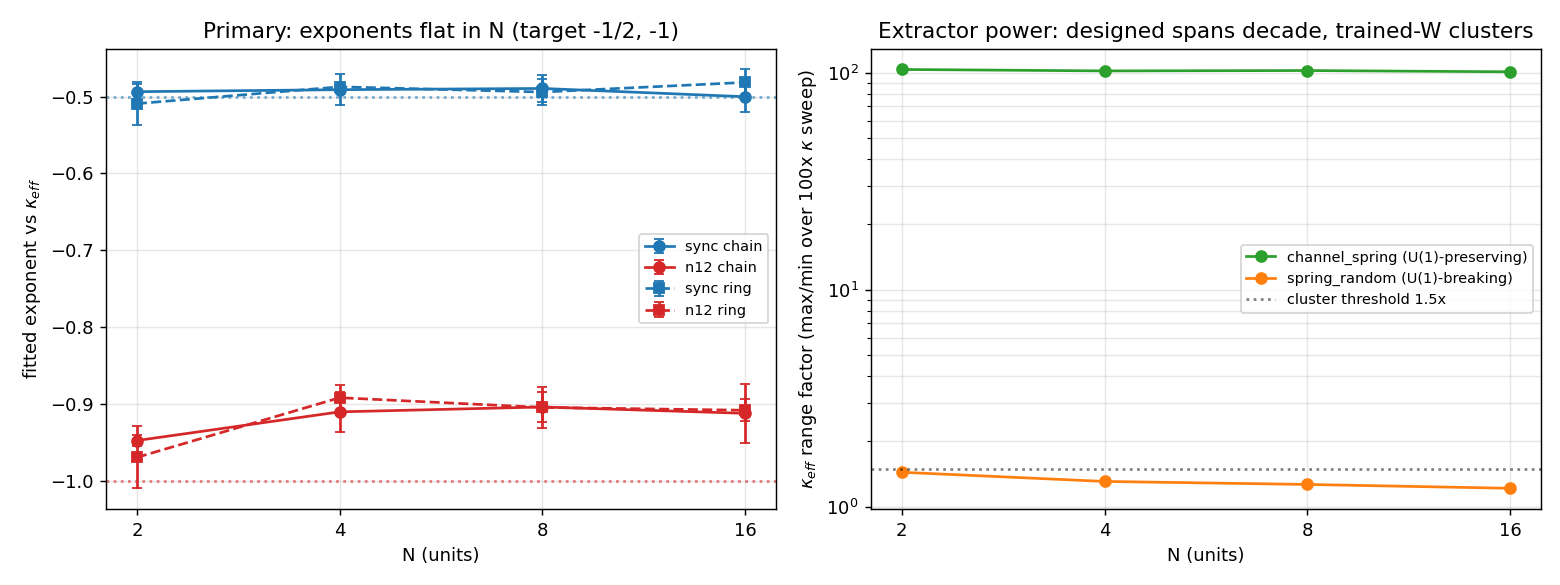
\includegraphics[width=0.72\linewidth]{figures/fig6_exponent_vs_N.png}
\caption{\textbf{[verification/control] The price-law exponents are flat in $N$; the $U(1)$-breaking control is unfittable.} Fitted sync and $n_{1/2}$ exponents vs lattice size $N\in\{2,4,8,16\}$ on the $U(1)$-preserving \texttt{channel\_spring} arm (chain and ring, $5$ seeds): both cluster on the theory's $-\tfrac12$/$-1$ with no monotonic drift (sync $-0.49\pm0.02$, $n_{1/2}$ $-0.91\pm0.03$, $R^2\ge0.998$). The \texttt{spring\_random} control (U(1)-breaking) is off-scale with $95\%$ CIs spanning $\pm12$ to $\pm887$ --- the direct cause of the former App.~C ``inconclusive,'' now resolved. Pre-registered decision rule applied verbatim. Source: \texttt{v3-pricing-n-scaling}.}
\label{fig:exponentN}
\end{figure}

\section{Metric discipline: why not the NTK cosine (CM-9 tail); and the resolved-spatial-structure panel}
The potential-NTK cosine $\cos\angle(\nabla_\theta V(q_A),\nabla_\theta V(q_B))\approx0.99$ for \emph{both} architectures (shared low-level features), hence uninformative. The firewall lives in the wake$-$sleep difference, where off-unit gradients cancel for the modular lattice and not for the monolith; $R_{B\leftarrow A}$ captures exactly this. Reviewers must use $R$, not the raw kernel.

\textbf{D.1 Spatial structure of $R$ (3 seeds, $N\in\{4,8\}$; \texttt{v3-interference-ntk} items 1/3).} Retained because it is the only place the \emph{spatial} structure (neighbour vs non-adjacent) is printed per-arm; its aggregate $S$ values are superseded, for the growth claim, by the 12-seed six-size measurement of \S3.2(ii).

\begin{center}\small
\begin{tabular}{lccc}
\toprule
config & $R_{\rm off}$ mean & $R_{\rm nn}$ (nbr) & $R_{\rm far}$ (non-adj) \\
\midrule
\textbf{modular} $N=4$ & $2.26\times10^{-5}$ & $4.53\times10^{-5}$ & $\mathbf{0.000}$ (exact) \\
\textbf{monolith} $N=4$ & $2.12\times10^{-1}$ & $2.42\times10^{-1}$ & $1.82\times10^{-1}$ \\
\textbf{modular} $N=8$ & $2.48\times10^{-5}$ & $9.92\times10^{-5}$ & $\mathbf{0.000}$ (exact) \\
\textbf{monolith} $N=8$ & $1.98\times10^{-1}$ & $1.78\times10^{-1}$ & $2.04\times10^{-1}$ \\
\bottomrule
\end{tabular}
\end{center}

\textbf{Reconciliation (no contradiction; C-7).} These are $3$-seed values ($\{0,1,2\}$); \S3.2 quotes $12$-seed values from a harness that reproduces this JSON \textbf{bit-exactly on the shared seeds and sizes} (max rel diff $0.00\times10^{0}$). The differences (per-edge leak $4.53\times10^{-5}$ here vs $\bar R_{\rm edge}=6.51\times10^{-5}$ at $N=4$ over 12 seeds) are seed sampling of an init-scale quantity with $\pm30\%$ scatter, not metric drift. \textbf{A negative worth recording (C-9):} on $3$ seeds the $N=4\to8$ \emph{growth factors} were modular $\times2.56$ vs monolith $\times2.18$ --- an apparent ``same slope, different offset'' reading. The per-seed $95\%$ CI on that modular growth factor is $\pm2.27$: the comparison was pure noise. With $12$ seeds the same window gives modular $\times1.36$ vs monolith $\times2.09$, and the full six-size slopes separate at $p=3.3\times10^{-4}$. Two-point scaling claims on a heavy-tailed init quantity are not claims; this is why \S3.2 leads with the exact structural identity and reports the growth claim only with $12$ seeds and six sizes.

\begin{figure}[t]
\centering
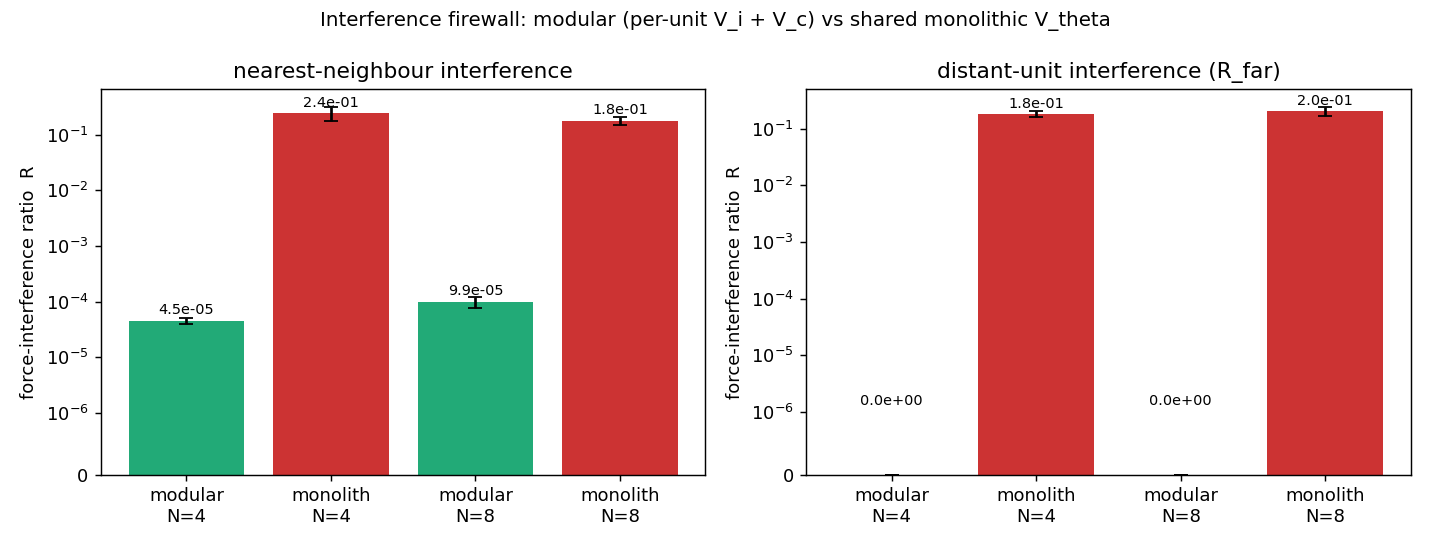
\includegraphics[width=0.68\linewidth]{figures/fig1_interference_bars.png}
\caption{\textbf{[evidence] Spatial structure of the interference kernel.} Cross-unit basin displacement $R$ resolved by graph distance for the modular lattice ($\approx10^{-5}$ neighbour, exactly zero non-adjacent) vs.\ the shared-potential monolith ($\approx0.2$, spatially unstructured: $R_{\rm nn}\approx R_{\rm far}$), $N\in\{4,8\}$, $3$ seeds, laptop-CPU (\texttt{v3-interference-ntk} items~1/3; aggregate growth superseded by Fig.~\ref{fig:interference}).}
\label{fig:bars}
\end{figure}

\section{The mass-lr inducer: full grid (CM-5; N7)}
$3$ seeds, 1500 ep, uniform init; \texttt{align}$=$Spearman(learned $M$, true band), \texttt{spread}$=$std(log $M$).
\begin{center}\small
\begin{tabular}{lllccc}
\toprule
$N$ & ratio & mult & align & log-spread & eval-MSE \\
\midrule
2 & 4$\times$ & 3 & $+1.00$ & 0.263 & 0.274 \\
2 & 4$\times$ & \textbf{10} & $+1.00$ & 0.553 & 0.033 \\
2 & 4$\times$ & 30 & $+1.00$ & 0.767 & 0.022 \\
2 & 4$\times$ & 100 & $+1.00$ & 1.171 & 0.373 \\
2 & 16$\times$ & 3 & $+1.00$ & 0.386 & 1.372 \\
2 & 16$\times$ & \textbf{10} & $+1.00$ & 0.488 & 0.633 \\
2 & 16$\times$ & 30 & $+0.33$ & 0.071 & 0.366 \\
2 & 16$\times$ & 100 & $-1.00$ & 0.176 & 0.332 \\
4 & 4$\times$ & 3 & $+1.00$ & 0.222 & 0.149 \\
4 & 4$\times$ & \textbf{10} & $+1.00$ & 0.442 & 0.028 \\
4 & 4$\times$ & 30 & $+1.00$ & 0.646 & 0.067 \\
4 & 4$\times$ & 100 & $+1.00$ & 1.718 & $35.27\pm47.26$ \\
4 & 16$\times$ & 3 & $+0.93$ & 0.347 & 0.680 \\
4 & 16$\times$ & \textbf{10} & $+0.80$ & 0.611 & 0.296 \\
4 & 16$\times$ & 30 & $+0.20$ & 0.678 & 0.197 \\
4 & 16$\times$ & 100 & $-0.20$ & 1.459 & 0.800 \\
\bottomrule
\end{tabular}
\end{center}
\textbf{N7:} the ``$\sim0.08$ ceiling / optimizer never finds it'' reading is a $300$-epoch budget artifact --- at $1500$ ep the uniform lattice orders masses correctly $5/5$ seeds (Spearman $+0.89$) and a $10\times$ mass-lr amplifies spread to $0.52$; but the designed magnitude is never reached (designed fits $7$--$14\times$ better). Ordering inducible; magnitude designed.

\section{Recovery ladder and loan curve (CM-1; C-9)}
\textbf{F.1 Loan curve (cumulative MSE, 3 seeds, \texttt{fit-gap-anatomy} item 2):}
\begin{center}\small
\begin{tabular}{lcccc}
\toprule
horizon & twin & chlu & broken\_vol & LSTM \\
\midrule
10 & $2.9\times10^{-6}$ & $2.2\times10^{-5}$ & $1.1\times10^{-4}$ & $7.5\times10^{-2}$ \\
100 & $2.4\times10^{-4}$ & $1.2\times10^{-2}$ & $4.1\times10^{-3}$ & $4.9\times10^{-2}$ \\
500 & $1.1\times10^{-2}$ & $1.8\times10^{-1}$ & $9.7\times10^{-2}$ & $7.7\times10^{-2}$ \\
1000 & $3.2\times10^{-1}$ & $\mathbf{2.0\times10^{-1}}$ & $1.2\times10^{-1}$ & $9.9\times10^{-2}$ \\
5000 & $\mathbf{1.96\times10^{2}}$ & $2.2\times10^{-1}$ & $1.4\times10^{-1}$ & $1.3\times10^{-1}$ \\
\bottomrule
\end{tabular}
\end{center}
Loan called between $500$ and $1000$ (crosses $\approx700$). CLU is not the lowest plateau (broken-vol $0.14$, LSTM $0.13 < $ CLU $0.22$); the asset is boundedness by construction. \textbf{F.2 Recovery ladder (\texttt{fit-gap-anatomy} item 3; twin gap $0.202$):} twin $0.0047$ (100\%); CLU $\gamma{=}0$ $0.2066$ (0\%, BIBO 1.00, drift 0.778, $\mu^2\,5.2\times10^{-3}$); \textbf{$+\gamma$ global $0.0216$ (92\%, all guarantees preserved)}; $+\gamma_\varphi$ $0.2548$ ($-24\%$, wrong lever). Reach rungs certificate-only: $+S^{(M)}$ $\det=1$ ($3\times10^{-7}$), inj $2.28\le e^2$, $\Delta q=2.18$; $+$inter-unit wormhole $\kappa{=}0$ bit-exact reduction re-verified.

\section{Prominent negatives registry (C-9)}
\textbf{N7} designed-not-emergent (ordering \emph{is} inducible) --- App~E. \textbf{N8} $100\times$ mass-lr inverts ordering --- App~B.3. \textbf{N9} slow-first curriculum did not help --- App~B.3. \textbf{N12} governor $+$ friction field do not compose (deploy the field alone). \textbf{N16} trained-coupling exponent was read ``inconclusive'' --- \textbf{now RESOLVED/re-attributed} (artifact of the \emph{learned} random-$W$ $U(1)$ breaking, not physics; on \texttt{channel\_spring} / designed $SO(2)$ units the exponent is verified flat across $N\le16$, $-0.49\pm0.02$/$-0.91\pm0.03$, pre-registered) --- \S3.3, Figs.~\ref{fig:pricinglaw}--\ref{fig:exponentN}, App~C. \textbf{N22} friction never stabilizes a saddle; governor blind to isoenergetic escape (theory note \S5) --- V3 assumes the licensed-contraction forgetting column. \textbf{Superseded internal measurement (process negative; App~D.1):} a $3$-seed, $2$-point ($N\in\{4,8\}$) reading of the interference growth suggested equal slopes ($\times2.56$ vs $\times2.18$); the per-seed $95\%$ CI on the modular factor was $\pm2.27$ --- the comparison carried no information. The $12$-seed six-size measurement reverses it ($\times1.36$ vs $\times2.09$; slopes diverge, $p=3.3\times10^{-4}$). \textbf{The firewall is not a physics result (App~H):} a block-diagonal potential with separate per-block parameters has $S\equiv0$ \emph{exactly} --- a strictly better firewall than our lattice's $\bar R_{\rm edge}\approx6.5\times10^{-5}$, with no Hamiltonian, no symplectic structure and no coupling graph. Nothing physics-specific buys interference confinement; what the lattice buys is a \emph{priced channel} through the firewall.

\section{The block-monolith and coordination-number controls (\S3.2(i),(iii))}
\emph{(Source: \texttt{v3-interference-extra}; flag-provenance A.2b. 12 seeds (block/scaling), 8 seeds (topology), $N\le16$, measured at initialization.)}

\textbf{H.1 Full five-arm block-monolith table.} A \textbf{single} potential $V:\R^{Nd}\to\R$ (one module; no lattice, no coupling graph, no Hamiltonian coupling) with an explicitly block-diagonal Hessian ($\partial^2V/\partial q_i\partial q_j=0$, $i\ne j$), in three parameter-sharing regimes, against the modular lattice and the naive monolith.

\begin{center}\footnotesize\setlength{\tabcolsep}{3pt}
\begin{tabular}{lccccccc}
\toprule
arm & params ($N{=}2{\to}16$) & $S(2)$ & $S(4)$ & $S(8)$ & $S(16)$ & per-pair $\bar R$ & $b$ over $[2,16]$ \\
\midrule
\textbf{block-untied} sep.\ $\theta_i$ & $2{,}370\to18{,}960$ & $\mathbf{0.0}$ & $\mathbf{0.0}$ & $\mathbf{0.0}$ & $\mathbf{0.0}$ & $\mathbf{0.0}$ & undef.\ ($S\equiv0$) \\
\textbf{modular} ($\kappa_c{=}0.05$) & $2{,}382\to19{,}112$ & $6.4\mathrm{e}{-5}$ & $9.8\mathrm{e}{-5}$ & $1.3\mathrm{e}{-4}$ & $1.1\mathrm{e}{-4}$ & ${\approx}6.5\mathrm{e}{-5}$ & $+0.46\pm0.31$ \\
block-trunk & $1{,}218\to1{,}680$ & $7.08\mathrm{e}{-2}$ & $2.20\mathrm{e}{-1}$ & $4.88\mathrm{e}{-1}$ & $1.05$ & $0.065$ & $+1.51\pm0.36$ \\
monolith & $1{,}253\to2{,}177$ & $2.18\mathrm{e}{-1}$ & $6.40\mathrm{e}{-1}$ & $1.34$ & $2.32$ & $0.19$ & $+1.18\pm0.17$ \\
\textbf{block-tied} (deep-sets) & $1{,}185$ (const.) & $9.64\mathrm{e}{-1}$ & $2.90$ & $6.78$ & $1.45\times10^{1}$ & $\mathbf{0.97}$ & $+1.29\pm0.01$ \\
\bottomrule
\end{tabular}
\end{center}

Exact-zero audit over all seeds/sizes (max off-diagonal $R$; nonzero far-field entries): modular $9.34\times10^{-4}$ / \textbf{0} of 4,656; \texttt{block\_untied} $0.000000\times10^{0}$ / \textbf{0}; monolith $6.22\times10^{-1}$ / 4,656; \texttt{block\_trunk} $3.50\times10^{-1}$ / 4,656; \texttt{block\_tied} $1.27$ / 4,656. Diagonal $R[A,A]=1.000000$ in all $72$ runs of every arm, so the \texttt{block\_untied} zero is genuine, not a degenerate normalization of a dead self-response. Readings: (a) \emph{block structure alone recovers nothing} (\texttt{block\_trunk} shares only a trunk and still leaks, $\bar R=0.065$, $b=+1.51$); (b) \emph{block structure $+$ disjoint parameters is a perfect firewall} ($S\equiv0$); (c) \emph{interference is not capacity} --- the $1{,}185$-parameter tied arm (constant in $N$) is worst, the $18{,}960$-parameter untied arm exactly zero, and \texttt{block\_tied}'s $S=14.5$ at $N=16$ is $129{,}033\times$ the modular value and $6.2\times$ the naive monolith; (d) the modular lattice equals \texttt{block\_untied} at $\kappa_c=0$ (measured $0.0$), so its ${\approx}6.5\times10^{-5}$ leak is precisely the price of having a coupling graph.

\begin{figure}[t]
\centering
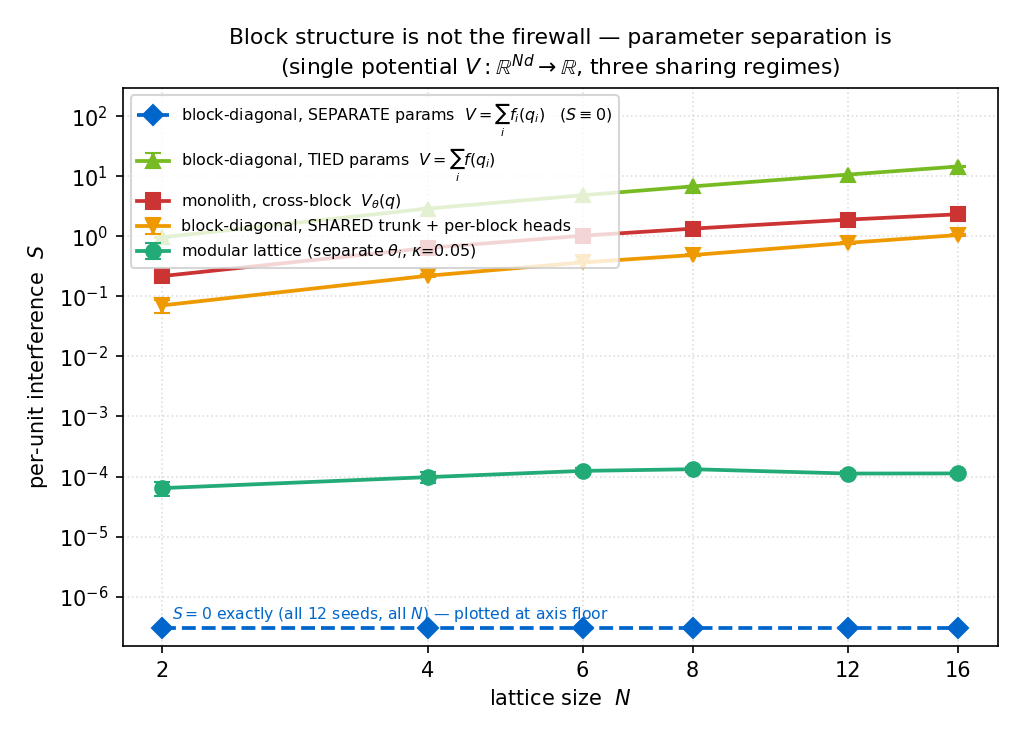
\includegraphics[width=0.72\linewidth]{figures/fig_block_monolith.png}
\caption{\textbf{[evidence] Parameter separation, not block structure, buys the firewall.} Per-unit received interference $S$ vs $N$ for five arms (12 seeds; log-$y$). \texttt{block\_untied} is drawn at the axis floor with an explicit ``$S=0$ exactly'' annotation; \texttt{block\_tied} (deep-sets, $1{,}185$ parameters constant in $N$) is the worst arm, above the naive monolith (\texttt{v3-interference-extra}).}
\label{fig:blockmono}
\end{figure}

\textbf{H.2 Coordination-number control (chain/ring/circulant-4).} 8 seeds; the identity $S=\deg\cdot\bar R_{\rm edge}$ holds to $S/(\deg\cdot\bar R_{\rm edge})=1.000000$ in \emph{every} cell:

\begin{center}\footnotesize\setlength{\tabcolsep}{4pt}
\begin{tabular}{lcccccc}
\toprule
topology & $N$ & mean degree & $S$ & $\bar R_{\rm edge}$ & $S/(\deg\cdot\bar R_{\rm edge})$ & non-edge nonzero \\
\midrule
chain & 4 & 1.50 & $7.934\times10^{-5}\pm3\times10^{-5}$ & $5.289\times10^{-5}$ & $1.000000$ & 0 \\
chain & 8 & 1.75 & $1.496\times10^{-4}\pm3\times10^{-5}$ & $8.549\times10^{-5}$ & $1.000000$ & 0 \\
chain & 16 & 1.88 & $1.148\times10^{-4}\pm4\times10^{-5}$ & $6.124\times10^{-5}$ & $1.000000$ & 0 \\
ring & 4 & 2.00 & $1.189\times10^{-4}\pm4\times10^{-5}$ & $5.944\times10^{-5}$ & $1.000000$ & 0 \\
ring & 8 & 2.00 & $1.724\times10^{-4}\pm5\times10^{-5}$ & $8.622\times10^{-5}$ & $1.000000$ & 0 \\
ring & 16 & 2.00 & $1.315\times10^{-4}\pm5\times10^{-5}$ & $6.575\times10^{-5}$ & $1.000000$ & 0 \\
circulant-4 & 8 & 4.00 & $2.829\times10^{-4}\pm8\times10^{-5}$ & $7.072\times10^{-5}$ & $1.000000$ & 0 \\
circulant-4 & 16 & 4.00 & $2.642\times10^{-4}\pm4\times10^{-5}$ & $6.605\times10^{-5}$ & $1.000000$ & 0 \\
\bottomrule
\end{tabular}
\end{center}

Slopes: chain $+0.264\pm0.171$ ($p=0.008$, a real end-effect from the degree ramp), ring $+0.071\pm0.183$ ($p=0.391$, flat), circulant-4 $-0.066\pm0.315$ ($p=0.636$, flat). Ring$\to$circulant-4 scales $S$ by $2.01\times$ at $N=16$ ($1.64\times$ at $N=8$); the shortfall at $N=8$ is $\bar R_{\rm edge}$ init scatter ($\pm30\%$ across lattices), \textbf{not} a degree effect --- the identity is exact per-run, so we quote the identity and never ``$2.0\times$'' as a measured constant.

\begin{figure}[t]
\centering
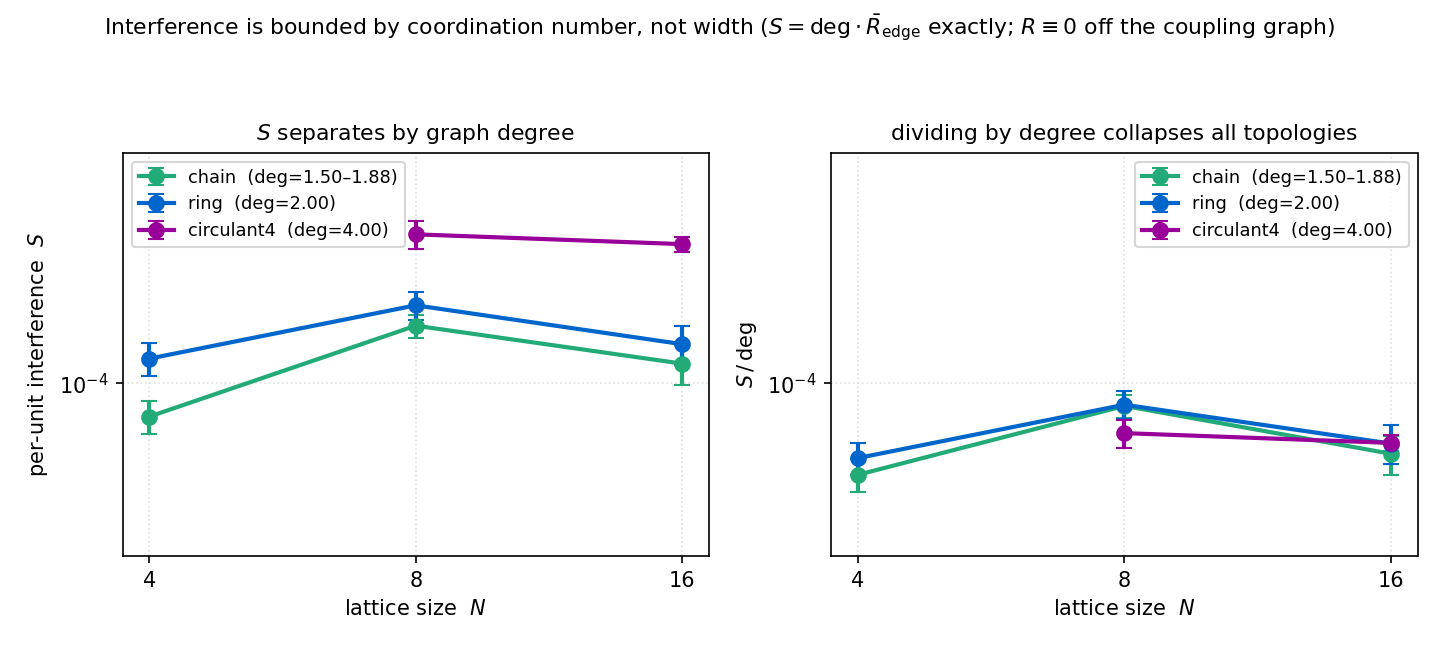
\includegraphics[width=0.95\linewidth]{figures/fig_coordination.png}
\caption{\textbf{[evidence] Interference is bounded by coordination number, not width.} (left) $S$ vs $N$ separates by graph degree (chain $1.50$--$1.88$, ring $2.00$, circulant-4 $4.00$); (right) dividing by degree collapses all three topologies. $R\equiv0$ off the coupling graph in every topology --- including the circulant, where graph distance and index distance disagree. 8 seeds, laptop-CPU (\texttt{v3-interference-extra}).}
\label{fig:coord}
\end{figure}

\textbf{H.3 Banding orthogonality, exact.} $\max|R_{\rm banded}-R_{\rm uniform}|=0.000\times10^{0}$ over $6$ sizes $\times$ $12$ seeds: the banded and uniform interference kernels are \textbf{bit-identical}, upgrading the earlier ``equal to every printed digit.'' $V_\theta$ has no \texttt{log\_mass} dependence; banding and the firewall are orthogonal knobs.

\section*{References (hermetic; C-8)}
\small\raggedright
\emph{Open bibliography slots (v0.4): three strings remain unresolved and are marked, never fabricated --- (a) Mo (2026); (b) Di Bernardo et al./Keller; (c) the checkpointing $O(\sqrt T)$ + RevNet/momentum-network anchors of the \S4 reversible paragraph. They were scheduled to land with the venue scout's bibliography sub-task, whose report does not exist at this revision.}\\[4pt]
Jawahar, P. \& Pierini, M. (2026). \emph{[CHLU reference --- the primitive's introduction].}\\
Anonymous (2026). \emph{The theory note} [F5 arXiv note; citation string pending live arXiv id].\\
Mo (2026). \emph{[Equivariant recurrent memory / Lyapunov-lifetime].}\\
Di Bernardo et al.; Keller. \emph{[Geometry-first structured recurrence].}\\
{}[$\cdot$] \emph{[Gradient checkpointing, $O(\sqrt T)$ memory]} --- marked slot, \S4.\\
{}[$\cdot$] \emph{[RevNet / momentum networks / reversible integrators]} --- marked slot, \S4.\\
McCloskey, M. \& Cohen, N. J. (1989). Catastrophic Interference in Connectionist Networks: The Sequential Learning Problem. \emph{Psychology of Learning and Motivation} 24, 109--165. doi:10.1016/S0079-7421(08)60536-8.\\
French, R. M. (1999). Catastrophic forgetting in connectionist networks. \emph{Trends in Cognitive Sciences} 3(4), 128--135. doi:10.1016/S1364-6613(99)01294-2.\\
Jacobs, R. A., Jordan, M. I., Nowlan, S. J. \& Hinton, G. E. (1991). Adaptive Mixtures of Local Experts. \emph{Neural Computation} 3(1), 79--87. doi:10.1162/neco.1991.3.1.79.\\
Shazeer, N., Mirhoseini, A., Maziarz, K., Davis, A., Le, Q., Hinton, G. \& Dean, J. (2017). Outrageously Large Neural Networks: The Sparsely-Gated Mixture-of-Experts Layer. \emph{ICLR 2017}. arXiv:1701.06538.\\
Kirkpatrick, J. et al. (2017). Overcoming catastrophic forgetting in neural networks. \emph{PNAS} 114(13), 3521--3526. arXiv:1612.00796.\\
Mallya, A. \& Lazebnik, S. (2018). PackNet: Adding Multiple Tasks to a Single Network by Iterative Pruning. \emph{CVPR 2018}, 7765--7773. arXiv:1711.05769.\\
Doan, T., Bennani, M. A., Mazoure, B., Rabusseau, G. \& Alquier, P. (2021). A Theoretical Analysis of Catastrophic Forgetting through the NTK Overlap Matrix. \emph{AISTATS 2021}, PMLR 130. arXiv:2010.04003.\\
Riemer, M., Cases, I., Ajemian, R., Liu, M., Rish, I., Tu, Y. \& Tesauro, G. (2019). Learning to Learn without Forgetting by Maximizing Transfer and Minimizing Interference. \emph{ICLR 2019}. arXiv:1810.11910.\\
Yu, T., Kumar, S., Gupta, A., Levine, S., Hausman, K. \& Finn, C. (2020). Gradient Surgery for Multi-Task Learning. \emph{NeurIPS 2020}. arXiv:2001.06782.\\
Boopathy, A., Jiang, S., Yue, W., Hwang, J., Iyer, A. \& Fiete, I. (2025). Breaking Neural Network Scaling Laws with Modularity. \emph{ICLR 2025}. arXiv:2409.05780.\\
Chen, Z., Zhang, J., Arjovsky, M. \& Bottou, L. (2020). Symplectic Recurrent Neural Networks. \emph{ICLR 2020}. arXiv:1909.13334.\\
Greydanus, S., Dzamba, M. \& Yosinski, J. (2019). Hamiltonian Neural Networks. \emph{NeurIPS 2019}. arXiv:1906.01563.\\
Cranmer, M., Greydanus, S., Hoyer, S., Battaglia, P., Spergel, D. \& Ho, S. (2020). Lagrangian Neural Networks. \emph{ICLR 2020 Workshop DeepDiffEq}. arXiv:2003.04630.\\
Erichson, N. B., Azencot, O., Queiruga, A., Hodgkinson, L. \& Mahoney, M. W. (2021). Lipschitz Recurrent Neural Networks. \emph{ICLR 2021}. arXiv:2006.12070.\\
Rusch, T. K. \& Mishra, S. (2021). Coupled Oscillatory Recurrent Neural Network (coRNN). \emph{ICLR 2021}. arXiv:2010.00951.\\
Rusch, T. K., Mishra, S., Erichson, N. B. \& Mahoney, M. W. (2022). Long Expressive Memory for Sequence Modeling. \emph{ICLR 2022}. arXiv:2110.04744.\\
Hochreiter, S. \& Schmidhuber, J. (1997). Long Short-Term Memory. \emph{Neural Computation} 9(8), 1735--1780. doi:10.1162/neco.1997.9.8.1735.\\
Hairer, E., Lubich, C. \& Wanner, G. (2006). \emph{Geometric Numerical Integration: Structure-Preserving Algorithms for ODEs} (2nd ed.). Springer SSCM 31.

\end{document}
